\documentclass[12pt]{article}\usepackage[]{graphicx}\usepackage[]{xcolor}
% maxwidth is the original width if it is less than linewidth
% otherwise use linewidth (to make sure the graphics do not exceed the margin)
\makeatletter
\def\maxwidth{ %
  \ifdim\Gin@nat@width>\linewidth
    \linewidth
  \else
    \Gin@nat@width
  \fi
}
\makeatother

\definecolor{fgcolor}{rgb}{0.345, 0.345, 0.345}
\newcommand{\hlnum}[1]{\textcolor[rgb]{0.686,0.059,0.569}{#1}}%
\newcommand{\hlstr}[1]{\textcolor[rgb]{0.192,0.494,0.8}{#1}}%
\newcommand{\hlcom}[1]{\textcolor[rgb]{0.678,0.584,0.686}{\textit{#1}}}%
\newcommand{\hlopt}[1]{\textcolor[rgb]{0,0,0}{#1}}%
\newcommand{\hlstd}[1]{\textcolor[rgb]{0.345,0.345,0.345}{#1}}%
\newcommand{\hlkwa}[1]{\textcolor[rgb]{0.161,0.373,0.58}{\textbf{#1}}}%
\newcommand{\hlkwb}[1]{\textcolor[rgb]{0.69,0.353,0.396}{#1}}%
\newcommand{\hlkwc}[1]{\textcolor[rgb]{0.333,0.667,0.333}{#1}}%
\newcommand{\hlkwd}[1]{\textcolor[rgb]{0.737,0.353,0.396}{\textbf{#1}}}%
\let\hlipl\hlkwb

\usepackage{framed}
\makeatletter
\newenvironment{kframe}{%
 \def\at@end@of@kframe{}%
 \ifinner\ifhmode%
  \def\at@end@of@kframe{\end{minipage}}%
  \begin{minipage}{\columnwidth}%
 \fi\fi%
 \def\FrameCommand##1{\hskip\@totalleftmargin \hskip-\fboxsep
 \colorbox{shadecolor}{##1}\hskip-\fboxsep
     % There is no \\@totalrightmargin, so:
     \hskip-\linewidth \hskip-\@totalleftmargin \hskip\columnwidth}%
 \MakeFramed {\advance\hsize-\width
   \@totalleftmargin\z@ \linewidth\hsize
   \@setminipage}}%
 {\par\unskip\endMakeFramed%
 \at@end@of@kframe}
\makeatother

\definecolor{shadecolor}{rgb}{.97, .97, .97}
\definecolor{messagecolor}{rgb}{0, 0, 0}
\definecolor{warningcolor}{rgb}{1, 0, 1}
\definecolor{errorcolor}{rgb}{1, 0, 0}
\newenvironment{knitrout}{}{} % an empty environment to be redefined in TeX

\usepackage{alltt}    % For submission



%% Package imports %%%%%%%%%%%%%%%%%%%%%%%%%%%%%%%%%%%%%%%%%%%

\usepackage{amsfonts}           % For access to \checkmark.
\usepackage{amsmath}            % For better symbol decorations
\usepackage{authblk}            % For a nice author block
\usepackage{booktabs}           % For nice table rules
\usepackage[official]{eurosym}  % For the euro symbol
\usepackage[figurename=Fig.]{caption} % For changing "Figure" to "Fig." in figure captions
\usepackage{chngcntr}           % To get figure and table numbering correct in the appendices
\usepackage[makeroom]{cancel}   % To show terms go to zero
\usepackage[inline]{enumitem}   % For inline enumeration
\usepackage[letterpaper, left=0.75in, right=0.75in, top=0.75in, bottom=0.75in, footskip=.25in]{geometry} % For better margins.
\usepackage[pagewise]{lineno}   % For line numbers
% \modulolinenumbers[5]
\usepackage{multicol}           % For multi-column layout
\usepackage{multirow}           % For multi-row layout
\usepackage{natbib}
\setlength{\bibsep}{0.0pt}      % To set the separation between entries to 0.
\usepackage{nccmath}            % For the \useshortskip command above equations
\usepackage{parcolumns}         % For multi-column layout
\usepackage{pdflscape}          % For landscape environment \begin{landscape} ... \end{landscape}
\usepackage{setspace}           % For double spacing
\doublespacing
\usepackage{soul}               % For text highlighting
\usepackage[most]{tcolorbox}    % For color highlighting of text
\usepackage{tikz}               % For diagrams
\usetikzlibrary{arrows,positioning}
\usepackage{ulem}               % For strikeout command (\sout)
\usepackage{xcolor}             % For ... colors

\usepackage{hyperref}           % hyperref should be the last package loaded


%% Macros defined by authors %%%%%%%%%%%%%%%%%%%%%%%%%%%%%%%%%

% The next command tells RStudio to do "Compile PDF" on HSB_framework.Rnw,
% instead of this file, thereby eliminating the need to switch back to HSB_framework.Rnw 
% before building the paper.
%!TEX root = ../HSB_framework.Rnw


%%%%%%%%%%%%%%%%%%%%%%%%%%%%%%%%%%%%%%%%%%%%%%%%%%%%%%%%%%%%%%
% This file contains macros for
% Heun, Semieniuk, Brockway, 
% Energy, expenditure, and consumption aspects of rebound,\\
% Part I: A rigorous analytical framework
% and
% Energy, expenditure, and consumption aspects of rebound,\\
% Part II: Applications of the framework
% 
% It is incorporated into the main file by the command
% % The next command tells RStudio to do "Compile PDF" on HSB_framework.Rnw,
% instead of this file, thereby eliminating the need to switch back to HSB_framework.Rnw 
% before building the paper.
%!TEX root = ../HSB_framework.Rnw


%%%%%%%%%%%%%%%%%%%%%%%%%%%%%%%%%%%%%%%%%%%%%%%%%%%%%%%%%%%%%%
% This file contains macros for
% Heun, Semieniuk, Brockway, 
% Energy, expenditure, and consumption aspects of rebound,\\
% Part I: A rigorous analytical framework
% and
% Energy, expenditure, and consumption aspects of rebound,\\
% Part II: Applications of the framework
% 
% It is incorporated into the main file by the command
% % The next command tells RStudio to do "Compile PDF" on HSB_framework.Rnw,
% instead of this file, thereby eliminating the need to switch back to HSB_framework.Rnw 
% before building the paper.
%!TEX root = ../HSB_framework.Rnw


%%%%%%%%%%%%%%%%%%%%%%%%%%%%%%%%%%%%%%%%%%%%%%%%%%%%%%%%%%%%%%
% This file contains macros for
% Heun, Semieniuk, Brockway, 
% Energy, expenditure, and consumption aspects of rebound,\\
% Part I: A rigorous analytical framework
% and
% Energy, expenditure, and consumption aspects of rebound,\\
% Part II: Applications of the framework
% 
% It is incorporated into the main file by the command
% \input{macros.tex}.
%%%%%%%%%%%%%%%%%%%%%%%%%%%%%%%%%%%%%%%%%%%%%%%%%%%%%%%%%%%%%%


%%%%% Override Energy Economics macros
\renewcommand{\emph}{\textit}


%%%%% Units

\newcommand{\kWhr}{kW$\cdot$hr}
\newcommand{\lmhr}{lm$\cdot$hr}
\newcommand{\passkm}{pass$\cdot$km}
\newcommand{\Whr}{W$\cdot$hr}


%%%%% Decorations for symbols

\newcommand{\rate}[1]{\dot{#1}}                    % Rate of a quantity

% Create "after" commands
\newcommand{\orig}[1]{{}{#1}^{\scriptscriptstyle \circ}}
\newcommand{\aempl}[1]{{#1}^*}
\newcommand{\asub}[1]{\hat{#1}}
\newcommand{\ainc}[1]{\bar{#1}}
\newcommand{\amacro}[1]{\tilde{#1}}

% Create the "before" commands
\newcommand{\bempl}[1]{\orig{#1}}
\newcommand{\bsub}[1]{\aempl{#1}}
\newcommand{\binc}[1]{\asub{#1}}
\newcommand{\bmacro}[1]{\ainc{#1}}

% Decoration combinations
% Rates after
\newcommand{\rorig}[1]{\orig{\rate{#1}}}
\newcommand{\raempl}[1]{\aempl{\rate{#1}}}
\newcommand{\rasub}[1]{\asub{\rate{#1}}}
\newcommand{\rainc}[1]{\ainc{\rate{#1}}}
\newcommand{\ramacro}[1]{\amacro{\rate{#1}}}

% Rates before
\newcommand{\rbempl}[1]{\rorig{#1}}
\newcommand{\rbsub}[1]{\raempl{#1}}
\newcommand{\rbinc}[1]{\rasub{#1}}
\newcommand{\rbmacro}[1]{\rainc{#1}}

%%%%% Subscript kerning

\newcommand{\om}{O\!M}
\newcommand{\omd}{O\!M\!d}
\newcommand{\md}{md}
\newcommand{\macro}{macr\!o}
\newcommand{\life}{li\!f\!e}
\newcommand{\EEU}{E\!EU}

%%%%% Expression kerning

\newcommand{\MPC}{M\!PC}


%%%%% Convenient symbols

\newcommand{\Sdot}{\rate{S}_{dev}}
\newcommand{\Mdothatprime}{\rbinc{M}^\prime}


%%%%% Elasticities and income shares

\newcommand{\eqspsUC}{\varepsilon_{\rate{q}_s\!,p_s}}
\newcommand{\eqopsUC}{\varepsilon_{\rate{q}_o\!,p_s}}
\newcommand{\eqspsC}{\varepsilon_{\rate{q}_s\!,p_s\!,c}}
\newcommand{\eqopsC}{\varepsilon_{\rate{q}_o\!,p_s\!,c}}

% originally
\newcommand{\eqspsUCorig}{\varepsilon^\circ_{\rate{q}_s\!,p_s}}
\newcommand{\eqopsUCorig}{\varepsilon^\circ_{\rate{q}_o\!,p_s}}
\newcommand{\eqspsCorig}{\varepsilon^\circ_{\rate{q}_s\!,p_s\!,c}}
\newcommand{\eqopsCorig}{\varepsilon^\circ_{\rate{q}_o\!,p_s\!,c}}
% With hats
\newcommand{\eqspsUChat}{\hat{\varepsilon}_{\rate{q}_s\!,p_s}}
\newcommand{\eqopsUChat}{\hat{\varepsilon}_{\rate{q}_o\!,p_s}}
\newcommand{\eqspsChat}{\hat{\varepsilon}_{\rate{q}_s\!,p_s\!,c}}
\newcommand{\eqopsChat}{\hat{\varepsilon}_{\rate{q}_o\!,p_s\!,c}}

\newcommand{\eqsM}{\varepsilon_{\rate{q}_s\!,\rate{M}}}
\newcommand{\eqoM}{\varepsilon_{\rate{q}_o\!,\rate{M}}}

\newcommand{\fCs}{\bempl{f}_{\rate{C}_s}}
\newcommand{\fCshat}{\asub{f}_{\rate{C}_s}}

\newcommand{\eQEpE}{\varepsilon_{\rate{Q}_E,p_E}}


%%%%% Colors

% Original spectrum colours
% \colorlet{emplcolor}{red!25!white}
% \colorlet{subcolor}{orange!25!white}
% \colorlet{inccolor}{green!25!white}
% \colorlet{macrocolor}{blue!25!white}

% New Viridis "plasma" colours
\definecolor{emplcolor}{HTML}{150789}
\definecolor{subcolor}{HTML}{99149F}
\definecolor{inccolor}{HTML}{E76F5A}
\definecolor{macrocolor}{HTML}{F7E225}



%%%%% Coloration of text background

%
% Inline color box around text
% Arguments:
%   [#1]: background color for the box
%   {#2}: text inside the box
%
\newtcbox{\inlinebox}[1][]{on line, 
colback=#1,
colframe=#1,
before upper={\rule[-2pt]{0pt}{10pt}},
boxrule=1pt,
boxsep=0pt,
left=3pt,
right=3pt,
top=2pt,
bottom=2pt}


%%%%% Colored phrases

% Emplacement effect
\newcommand{\empleffect}{\inlinebox[emplcolor]{\textcolor{white}{emplacement effect}}}
\newcommand{\empleffectadj}{\inlinebox[emplcolor]{\textcolor{white}{emplacement-effect}}}
\newcommand{\Empleffect}{\inlinebox[emplcolor]{\textcolor{white}{Emplacement effect}}}
\newcommand{\EmplEffect}{\inlinebox[emplcolor]{\textcolor{white}{Emplacement Effect}}}

% Substitution effect
\newcommand{\subeffect}{\inlinebox[subcolor]{\textcolor{white}{substitution effect}}}
\newcommand{\subeffectadj}{\inlinebox[subcolor]{\textcolor{white}{substitution-effect}}}
\newcommand{\Subeffect}{\inlinebox[subcolor]{\textcolor{white}{Substitution effect}}}
\newcommand{\SubEffect}{\inlinebox[subcolor]{\textcolor{white}{Substitution Effect}}}

% Income effect
\newcommand{\inceffect}{\inlinebox[inccolor]{\textcolor{black}{income effect}}}
\newcommand{\inceffectadj}{\inlinebox[inccolor]{\textcolor{black}{income-effect}}}
\newcommand{\Inceffect}{\inlinebox[inccolor]{\textcolor{black}{Income effect}}}
\newcommand{\IncEffect}{\inlinebox[inccolor]{\textcolor{black}{Income Effect}}}

% Macro effect
\newcommand{\macroeffect}{\inlinebox[macrocolor]{\textcolor{black}{macro effect}}}
\newcommand{\macroeffectadj}{\inlinebox[macrocolor]{\textcolor{black}{macro-effect}}}
\newcommand{\Macroeffect}{\inlinebox[macrocolor]{\textcolor{black}{Macro effect}}}
\newcommand{\MacroEffect}{\inlinebox[macrocolor]{\textcolor{black}{Macro Effect}}}


%%%%% minipage for assumptions and constraints tables
% Arguments:
%   #1: Width (multiple of \linewidth
%   #2: text inside the minipage
%
\newcommand{\mptable}[2]{\begin{minipage}{#1\linewidth} \useshortskip{} \begin{equation} #2 \end{equation} \end{minipage}}


%%%%% Oft-used references

\newcommand{\Ba}[1]{\citeauthor[#1]{Borenstein:2015aa}}
\newcommand{\Bapp}[1]{\citeauthor[#1]{Borenstein:2015aa}'s \citeyearpar{Borenstein:2015aa}}
\newcommand{\Bp}[1]{\citep[#1]{Borenstein:2015aa}}
\newcommand{\Bt}[1]{\citet[#1]{Borenstein:2015aa}}

\newcommand{\Ta}[1]{\citeauthor[#1]{Thomas:2013aa}}
\newcommand{\Tapp}[1]{\citeauthor[#1]{Thomas:2013aa}'s \citeyearpar{Thomas:2013aa}}
\newcommand{\Tp}[1]{\citep[#1]{Thomas:2013aa, Thomas:2013ab}}
\newcommand{\Tpone}[1]{\citep[#1]{Thomas:2013aa}}
\newcommand{\Tptwo}[1]{\citep[#1]{Thomas:2013ab}}
\newcommand{\Tt}[1]{\citet[#1]{Thomas:2013aa, Thomas:2013ab}}
\newcommand{\Ttone}[1]{\citet[#1]{Thomas:2013aa}}
\newcommand{\Tttwo}[1]{\citet[#1]{Thomas:2013ab}}


%%%%% Derivation pages

% Column widths
\newcommand{\derivtextsize}{\footnotesize}
\newcommand{\derivpageleftcolwidth}{0.11\textwidth}
\newcommand{\derivpageenergycolwidth}{0.6\textwidth}
\newcommand{\derivpagefinancialcolwidth}{0.6\textwidth}

% Horizontal rule between sections of derivations

\newcommand{\sectionsep}{\noindent\rule{1.4\textwidth}{0.4pt}}


%
% Derivation section
% Arguments:
%   #1: accounting stage (original, prime, etc.)
%   #2: energy column
%   #3: financial column
%
\newcommand{\derivsection}[3]{%

\derivtextsize{}

\begin{minipage}[t]{\derivpageleftcolwidth}
~\\#1
\end{minipage}
%
%
%
\begin{minipage}[t]{\derivpageenergycolwidth}
#2
\end{minipage}
%
~
%
\begin{minipage}[t]{\derivpagefinancialcolwidth}
#3
\end{minipage}

\normalsize{}

}


%
% Derivation page header
% Arguments:
%   #1: Effect type header text (e.g., Emplacement Effect)
%
\newcommand{\derivheader}[1]{

\begin{center}
  #1
\end{center}

\derivsection{}
{\begin{center}\emph{Energy analysis}\end{center}}
{\begin{center}\emph{Financial analysis}\end{center}}

}


% Equations

% Efficiency ratios
\newcommand{\etaratioinline}{\amacro{\eta}/\bempl{\eta}}
\newcommand{\etaratiostacked}{\frac{\amacro{\eta}}{\bempl{\eta}}}

% Derivative with respect to efficiency ratio
\newcommand{\dbydetaeta}{\frac{\mathrm{d}}{\mathrm{d}(\etaratioinline{})}}


% Original
\newcommand{\Eacctorig}{\rbempl{E} = \rbempl{E}_s + \rbempl{E}_{emb} + (\rbempl{C}_{\omd} + \rbempl{C}_o) I_E}
\newcommand{\Macctorig}{\rate{M} = p_E \rbempl{E}_s + \bempl{R}_\alpha \rbempl{C}_{cap} + \rbempl{C}_{\omd} + \rbempl{C}_o + \rbempl{N}}

% Before emplacement effect (same as original)
\newcommand{\Eacctbempl}{\Eacctorig}      
\newcommand{\Macctbempl}{\Macctorig}      

% After emplacement effect
\newcommand{\Eacctaempl}{\raempl{E} = \raempl{E}_s + \raempl{E}_{emb} + (\raempl{C}_{\omd} + \raempl{C}_o) I_E}                  
\newcommand{\Macctaempl}{\rate{M} = p_E \raempl{E}_s + \aempl{R}_\alpha \raempl{C}_{cap} + \raempl{C}_{\omd} + \raempl{C}_o + \raempl{N}}         

% Before substitution effect (same as after emplacement effect)
\newcommand{\Eacctbsub}{\Eacctaempl}
\newcommand{\Macctbsub}{\Macctaempl}

% After substitution effect
\newcommand{\Eacctasub}{\rasub{E} = \rasub{E}_s + \rasub{E}_{emb} + (\rasub{C}_{\omd} + \rasub{C}_o) I_E}
\newcommand{\Macctasub}{\rate{M} = p_E \rasub{E}_s + \asub{R}_\alpha \rasub{C}_{cap} + \rasub{C}_{\omd} + \rasub{C}_o + \rasub{N}}

% Before income effect (same as after substitution effect)
\newcommand{\Eacctbinc}{\Eacctasub}
\newcommand{\Macctbinc}{\Macctasub}

% After income effect
\newcommand{\Eacctainc}{\rainc{E} = \rainc{E}_s + \rainc{E}_{emb} + (\rainc{C}_{\omd} + \rainc{C}_o) I_E}
\newcommand{\Macctainc}{\rate{M} = p_E \rainc{E}_s + \ainc{R}_\alpha \rainc{C}_{cap} + \rainc{C}_{\omd} + \rainc{C}_o + \rainc{N}}

% Embodied energy rebound
\newcommand{\Reembeqn}{\frac{\left( \frac{\aempl{E}_{emb}}{\bempl{E}_{emb}}
  \frac{\bempl{t}_{\life}}{\aempl{t}_{\life}} - 1 \right) \rbempl{E}_{emb}}{\Sdot}}
  
% Ops, Maintenance, and disposal energy rebound
\newcommand{\ReOMdeqn}{\frac{\left( \frac{\raempl{C}_{\omd}}{\rbempl{C}_{\omd}} - 1 \right) \rbempl{C}_{\omd} I_E}{\Sdot}}

% Equation for S_dot_dev
% \newcommand{\Sdoteqn}{\left( \etaratiostacked - 1 \right)\!\etaratiostacked \rbempl{E}_s}
\newcommand{\Sdoteqn}{\left( \etaratiostacked - 1 \right)\! 
                            \frac{\bempl{\eta}}{\amacro{\eta}} \rbempl{E}_s}

% Equation for Re_dsub
\newcommand{\Redsubeqn}{\frac{\left( \etaratiostacked \right)^{-\eqspsUC} - 1}
                        {\etaratiostacked - 1}}
                        
% Equation for Re_isub
\newcommand{\Reisubeqn}{\frac{{\left( \etaratiostacked  \right)}
                          ^{-\eqopsC} - 1}{\etaratiostacked - 1} \; 
                          \etaratiostacked \; 
                          \frac{\rbempl{C}_o I_E}{\rbempl{E}_s}}
                          
% CES utility equation
\newcommand{\cesutility}{\left[ \fCs \left( \frac{\rate{q}_s}{\rbempl{q}_s} \right)^\rho 
        + (1-\fCs) \left( \frac{\rate{C}_o}{\rbempl{C}_o} \right)^\rho  \right]^{(1/\rho)}}
        
% Equation for q_s_hat/q_s_orig
\newcommand{\qssolution}{\left\{ \fCs + (1-\fCs)
      \left[ \left(  \frac{1-\fCs}{\fCs}  \right) \frac{\amacro{p}_s \rbempl{q}_s}{\rbempl{C}_o}  \right]
                                                  ^{\rho / (1 - \rho)} \right\} ^ {-1/\rho}}

% Equation for C_o_hat/C_o_orig
\newcommand{\Cosolution}{ \left( 1 + \fCs \left\{ \left[ \left( \frac{1-\fCs}{\fCs} \right)
          \frac{\amacro{p}_s \rbempl{q}_s}{\rbempl{C}_o} \right] ^{\rho/(\rho - 1)} - 1 \right\} \right)^{-1/\rho}}

% Equation for Re_dsub for the CES utility model
\newcommand{\RedsubCES}{\frac{\qssolution{} - 1}{\etaratiostacked{} - 1}}

% Equation for Re_isub for the CES utility model
\newcommand{\ReisubCES}{\frac{\Cosolution{} - 1}{\etaratiostacked{} - 1}
                         \etaratiostacked \; 
                          \frac{\rbempl{C}_o I_E}{\rbempl{E}_s}}


% Equation for Re_dinc, approximate method
\newcommand{\Redinceqnapprox}{\frac{ \left( 1 + \frac{\rbinc{N}}{\Mdothatprime} \right) ^{\eqsM} - 1}
              { \etaratiostacked - 1 } \left( \etaratiostacked \right)^{-\eqspsC}}

% Equation for Re_dinc, exact method
\newcommand{\Redinceqnexact}{\frac{ \left( 1 + \frac{\rbinc{N}}{\Mdothatprime} \right) ^{\eqsM} - 1}
              { \etaratiostacked - 1 } \qssolution{} }

% Equation for Re_cap
\newcommand{\Recapeqn}{\frac{\Delta \aempl{(R_\alpha \rate{C}_{cap})} I_E}{\Sdot}}

% Equation for Re_iinc, approximate method
\newcommand{\Reiinceqnapprox}{\frac{\left( 1 + \frac{\rbinc{N}}{\Mdothatprime} \right)^{\eqoM} - 1}{\etaratiostacked - 1} 
              \left( \etaratiostacked \right)^{1 - \eqopsC}
              \frac{\rbempl{C}_o I_E}{\rbempl{E}_s}}

% Equation for Re_iinc, exact method
% \newcommand{\Reiinceqnexact}{\frac{\left( 1 + \frac{\rbinc{N}}{\Mdothatprime} \right)^{\eqoM} - 1}{\etaratiostacked - 1} 
%               \left( \etaratiostacked \right)
%               \left( \frac{\rasub{C}_o}{\rorig{C}_o} \right) 
%               \frac{\rbempl{C}_o I_E}{\rbempl{E}_s}}

\newcommand{\Reiinceqnexact}{\frac{\left( 1 + \frac{\rbinc{N}}{\Mdothatprime} \right)^{\eqoM} - 1}{\etaratiostacked - 1} 
              \left( \etaratiostacked \right)
              \frac{\rbempl{C}_o I_E}{\rbempl{E}_s}
              \Cosolution{}}



% Equation for Re_d (total direct rebound)
\newcommand{\Redeqn}{\frac{ \left( \etaratiostacked \right)^{-\eqspsC}
             \left( 1 + \frac{\rasub{N}}{\rbempl{M}} \right)^{\eqsM}   - 1}
         {\etaratiostacked - 1}}

% Equation for Re_macro
% \newcommand{\Remacroeqn}{k (p_E I_E - Re_{cap} - Re_{\md} - p_E I_E Re_{dsub} - Re_{isub})}
\newcommand{\Remacroeqn}{k (p_E I_E - Re_{cap} - Re_{\omd})}

% Equation for Re_tot
% \newcommand{\Retoteqn}{&Re_{emb} - k Re_{cap} + (1-k) Re_{\md}         \nonumber \\
%                        &+ (1 - k p_E I_E) Re_{dsub} + (1 - k) Re_{isub}   \nonumber \\
%                        &+ Re_{dinc} + Re_{iinc} +  k p_E I_E}
% \newcommand{\Retoteqn}{&Re_{emb} + k (p_E I_E - Re_{cap}) + (1-k) Re_{\md}   \nonumber \\
%                        &+ Re_{dsub} + Re_{isub}                              \nonumber \\
%                        &+ Re_{dinc} + Re_{iinc}}
\newcommand{\Retoteqn}{Re_{emb} + k (p_E I_E - Re_{cap}) + (1-k) Re_{\omd} + Re_{dsub} + Re_{isub} + Re_{dinc} + Re_{iinc}}
                 

%%%% Income preference equations

% Equation for energy service income preferences
\newcommand{\incprefseqn}{\frac{\rainc{q}_s}{\rbinc{q}_s} = \left( 1 + \frac{\rbinc{N}}{\Mdothatprime}  \right) ^{\eqsM}}

% Equation for other goods income preferences
\newcommand{\incprefoeqn}{\frac{\rainc{q}_o}{\rbinc{q}_o} = \left( 1 + \frac{\rbinc{N}}{\Mdothatprime}  \right) ^{\eqoM}}

% Equation for effective income
% \newcommand{\effinceqn}{\Mdothatprime \equiv \rbempl{M} - \rbempl{C}_{cap} - \rbempl{C}_{\md} 
%                         - \rate{G} + p_E \Delta \rbinc{E}_s + \Delta \rbinc{C}_o}
\newcommand{\effinceqn}{\Mdothatprime \equiv \rate{M} - \aempl{R}_\alpha \raempl{C}_{cap} - \raempl{C}_{\omd} - \rasub{N}}


%%%% Budget constraint symbols and equation

\newcommand{\tlife}{t_{li\!f\!e}}
\newcommand{\oneyr}{1\,\mathrm{yr}}
\newcommand{\twoyr}{2\,\mathrm{yr}}
\newcommand{\itlife}{i\,t_{li\!f\!e}}
\newcommand{\iyr}{i\,\mathrm{yr}}

\newcommand{\budgetconstraint}{\rate{M} - \orig{R}_\alpha \rorig{C}_{cap} - \rorig{C}_{\omd} = \orig{p}_E \frac{\rorig{q}_s}{\orig{\eta}} + p_o \rorig{q}_o}


%%%% Proof characters
% Equal sign with question mark above
\DeclareRobustCommand{\questionequal}{\stackrel{?}{=}}




% Segments and lines
% Arguments:
%   #1: left character
%   #2: line color
%   #3: line thickness (e.g., 0.1 mm)
%   #4: right character
% Note that \raisebox{0.9 mm} moves the line up from the baseline.
% Also, \line(1,0){12} gives a horizontal line with length "12" (unknown units!)
% (1, 0) is the slope (1 unit to right, 0 units up).
\newcommand{\seg}[4]{#1\linethickness{#3}\raisebox{0.88 mm}{\textcolor{#2}{\line(1,0){12}}}#4}

% Construction lines
\newcommand{\iicirc}{\seg{$\bempl{\text{i}}$}{black}{0.3 mm}{$\,\bempl{\text{i}}$}}
\newcommand{\iibar}{\seg{$\bmacro{\text{i}}$}{black}{0.3 mm}{$\,\bmacro{\text{i}}$}}
\newcommand{\rr}{\seg{r}{black}{0.1 mm}{r}}
\newcommand{\circcirc}{\seg{$\circ$}{black}{0.1 mm}{$\circ$}}
\newcommand{\starstar}{\seg{$*$}{black}{0.1 mm}{$*$}}
\newcommand{\hathat}{\seg{$\wedge$}{black}{0.1 mm}{$\wedge$}}
\newcommand{\barbar}{\seg{$-\,$}{black}{0.1 mm}{$\, -$}}

% Line segments
\newcommand{\circa}{\seg{$\circ$}{emplcolor}{0.6 mm}{$a$}}
% \newcommand{\ab}{\seg{a}{emplcolor}{0.6 mm}{b}}
\newcommand{\ab}{$a$\tikz[baseline=-0.6ex]\draw [line width=0.6mm,dotted,emplcolor] (0,0) -- (0.45,0);$b$}
\newcommand{\bstar}{\seg{$b\,$}{emplcolor}{0.6 mm}{$*$}}
\newcommand{\starc}{\seg{$*$}{subcolor}{0.6 mm}{$\,c$}}
\newcommand{\chat}{\seg{$c\,$}{subcolor}{0.6 mm}{$\wedge$}}
\newcommand{\hatd}{\seg{$\wedge$}{inccolor}{0.6 mm}{$\,d$}}
\newcommand{\dbar}{\seg{$d$}{inccolor}{0.6 mm}{$\,-$}}
\newcommand{\hatbar}{\seg{$\wedge$}{inccolor}{0.6 mm}{$\,-$}}
\newcommand{\bartilde}{\seg{$- \,$}{macrocolor}{0.6 mm}{$\, \sim$}}


% Rotated text for tables
% See
% https://tex.stackexchange.com/questions/98388/how-to-make-table-with-rotated-table-headers-in-latex/98439#98439
% for details.
\newcommand{\rot}{\rotatebox{90}}


% A "rating" command for filled circles with tikz.
% See 
% https://tex.stackexchange.com/questions/194955/get-partly-filled-circle-symbol-scale-linearly-with-parameter
% for details.
\newcommand{\rating}[2][0.75ex]{%
  \pgfmathsetmacro\th{asin(#2/50-1)}% (theta angle of polar coordinates)
    \tikz{%
      \fill[black] (\th:#1) arc (\th:-180-\th:#1) -- cycle;
      \draw[black, thin, radius=#1] (0,0) circle;
    }%
}.
%%%%%%%%%%%%%%%%%%%%%%%%%%%%%%%%%%%%%%%%%%%%%%%%%%%%%%%%%%%%%%


%%%%% Override Energy Economics macros
\renewcommand{\emph}{\textit}


%%%%% Units

\newcommand{\kWhr}{kW$\cdot$hr}
\newcommand{\lmhr}{lm$\cdot$hr}
\newcommand{\passkm}{pass$\cdot$km}
\newcommand{\Whr}{W$\cdot$hr}


%%%%% Decorations for symbols

\newcommand{\rate}[1]{\dot{#1}}                    % Rate of a quantity

% Create "after" commands
\newcommand{\orig}[1]{{}{#1}^{\scriptscriptstyle \circ}}
\newcommand{\aempl}[1]{{#1}^*}
\newcommand{\asub}[1]{\hat{#1}}
\newcommand{\ainc}[1]{\bar{#1}}
\newcommand{\amacro}[1]{\tilde{#1}}

% Create the "before" commands
\newcommand{\bempl}[1]{\orig{#1}}
\newcommand{\bsub}[1]{\aempl{#1}}
\newcommand{\binc}[1]{\asub{#1}}
\newcommand{\bmacro}[1]{\ainc{#1}}

% Decoration combinations
% Rates after
\newcommand{\rorig}[1]{\orig{\rate{#1}}}
\newcommand{\raempl}[1]{\aempl{\rate{#1}}}
\newcommand{\rasub}[1]{\asub{\rate{#1}}}
\newcommand{\rainc}[1]{\ainc{\rate{#1}}}
\newcommand{\ramacro}[1]{\amacro{\rate{#1}}}

% Rates before
\newcommand{\rbempl}[1]{\rorig{#1}}
\newcommand{\rbsub}[1]{\raempl{#1}}
\newcommand{\rbinc}[1]{\rasub{#1}}
\newcommand{\rbmacro}[1]{\rainc{#1}}

%%%%% Subscript kerning

\newcommand{\om}{O\!M}
\newcommand{\omd}{O\!M\!d}
\newcommand{\md}{md}
\newcommand{\macro}{macr\!o}
\newcommand{\life}{li\!f\!e}
\newcommand{\EEU}{E\!EU}

%%%%% Expression kerning

\newcommand{\MPC}{M\!PC}


%%%%% Convenient symbols

\newcommand{\Sdot}{\rate{S}_{dev}}
\newcommand{\Mdothatprime}{\rbinc{M}^\prime}


%%%%% Elasticities and income shares

\newcommand{\eqspsUC}{\varepsilon_{\rate{q}_s\!,p_s}}
\newcommand{\eqopsUC}{\varepsilon_{\rate{q}_o\!,p_s}}
\newcommand{\eqspsC}{\varepsilon_{\rate{q}_s\!,p_s\!,c}}
\newcommand{\eqopsC}{\varepsilon_{\rate{q}_o\!,p_s\!,c}}

% originally
\newcommand{\eqspsUCorig}{\varepsilon^\circ_{\rate{q}_s\!,p_s}}
\newcommand{\eqopsUCorig}{\varepsilon^\circ_{\rate{q}_o\!,p_s}}
\newcommand{\eqspsCorig}{\varepsilon^\circ_{\rate{q}_s\!,p_s\!,c}}
\newcommand{\eqopsCorig}{\varepsilon^\circ_{\rate{q}_o\!,p_s\!,c}}
% With hats
\newcommand{\eqspsUChat}{\hat{\varepsilon}_{\rate{q}_s\!,p_s}}
\newcommand{\eqopsUChat}{\hat{\varepsilon}_{\rate{q}_o\!,p_s}}
\newcommand{\eqspsChat}{\hat{\varepsilon}_{\rate{q}_s\!,p_s\!,c}}
\newcommand{\eqopsChat}{\hat{\varepsilon}_{\rate{q}_o\!,p_s\!,c}}

\newcommand{\eqsM}{\varepsilon_{\rate{q}_s\!,\rate{M}}}
\newcommand{\eqoM}{\varepsilon_{\rate{q}_o\!,\rate{M}}}

\newcommand{\fCs}{\bempl{f}_{\rate{C}_s}}
\newcommand{\fCshat}{\asub{f}_{\rate{C}_s}}

\newcommand{\eQEpE}{\varepsilon_{\rate{Q}_E,p_E}}


%%%%% Colors

% Original spectrum colours
% \colorlet{emplcolor}{red!25!white}
% \colorlet{subcolor}{orange!25!white}
% \colorlet{inccolor}{green!25!white}
% \colorlet{macrocolor}{blue!25!white}

% New Viridis "plasma" colours
\definecolor{emplcolor}{HTML}{150789}
\definecolor{subcolor}{HTML}{99149F}
\definecolor{inccolor}{HTML}{E76F5A}
\definecolor{macrocolor}{HTML}{F7E225}



%%%%% Coloration of text background

%
% Inline color box around text
% Arguments:
%   [#1]: background color for the box
%   {#2}: text inside the box
%
\newtcbox{\inlinebox}[1][]{on line, 
colback=#1,
colframe=#1,
before upper={\rule[-2pt]{0pt}{10pt}},
boxrule=1pt,
boxsep=0pt,
left=3pt,
right=3pt,
top=2pt,
bottom=2pt}


%%%%% Colored phrases

% Emplacement effect
\newcommand{\empleffect}{\inlinebox[emplcolor]{\textcolor{white}{emplacement effect}}}
\newcommand{\empleffectadj}{\inlinebox[emplcolor]{\textcolor{white}{emplacement-effect}}}
\newcommand{\Empleffect}{\inlinebox[emplcolor]{\textcolor{white}{Emplacement effect}}}
\newcommand{\EmplEffect}{\inlinebox[emplcolor]{\textcolor{white}{Emplacement Effect}}}

% Substitution effect
\newcommand{\subeffect}{\inlinebox[subcolor]{\textcolor{white}{substitution effect}}}
\newcommand{\subeffectadj}{\inlinebox[subcolor]{\textcolor{white}{substitution-effect}}}
\newcommand{\Subeffect}{\inlinebox[subcolor]{\textcolor{white}{Substitution effect}}}
\newcommand{\SubEffect}{\inlinebox[subcolor]{\textcolor{white}{Substitution Effect}}}

% Income effect
\newcommand{\inceffect}{\inlinebox[inccolor]{\textcolor{black}{income effect}}}
\newcommand{\inceffectadj}{\inlinebox[inccolor]{\textcolor{black}{income-effect}}}
\newcommand{\Inceffect}{\inlinebox[inccolor]{\textcolor{black}{Income effect}}}
\newcommand{\IncEffect}{\inlinebox[inccolor]{\textcolor{black}{Income Effect}}}

% Macro effect
\newcommand{\macroeffect}{\inlinebox[macrocolor]{\textcolor{black}{macro effect}}}
\newcommand{\macroeffectadj}{\inlinebox[macrocolor]{\textcolor{black}{macro-effect}}}
\newcommand{\Macroeffect}{\inlinebox[macrocolor]{\textcolor{black}{Macro effect}}}
\newcommand{\MacroEffect}{\inlinebox[macrocolor]{\textcolor{black}{Macro Effect}}}


%%%%% minipage for assumptions and constraints tables
% Arguments:
%   #1: Width (multiple of \linewidth
%   #2: text inside the minipage
%
\newcommand{\mptable}[2]{\begin{minipage}{#1\linewidth} \useshortskip{} \begin{equation} #2 \end{equation} \end{minipage}}


%%%%% Oft-used references

\newcommand{\Ba}[1]{\citeauthor[#1]{Borenstein:2015aa}}
\newcommand{\Bapp}[1]{\citeauthor[#1]{Borenstein:2015aa}'s \citeyearpar{Borenstein:2015aa}}
\newcommand{\Bp}[1]{\citep[#1]{Borenstein:2015aa}}
\newcommand{\Bt}[1]{\citet[#1]{Borenstein:2015aa}}

\newcommand{\Ta}[1]{\citeauthor[#1]{Thomas:2013aa}}
\newcommand{\Tapp}[1]{\citeauthor[#1]{Thomas:2013aa}'s \citeyearpar{Thomas:2013aa}}
\newcommand{\Tp}[1]{\citep[#1]{Thomas:2013aa, Thomas:2013ab}}
\newcommand{\Tpone}[1]{\citep[#1]{Thomas:2013aa}}
\newcommand{\Tptwo}[1]{\citep[#1]{Thomas:2013ab}}
\newcommand{\Tt}[1]{\citet[#1]{Thomas:2013aa, Thomas:2013ab}}
\newcommand{\Ttone}[1]{\citet[#1]{Thomas:2013aa}}
\newcommand{\Tttwo}[1]{\citet[#1]{Thomas:2013ab}}


%%%%% Derivation pages

% Column widths
\newcommand{\derivtextsize}{\footnotesize}
\newcommand{\derivpageleftcolwidth}{0.11\textwidth}
\newcommand{\derivpageenergycolwidth}{0.6\textwidth}
\newcommand{\derivpagefinancialcolwidth}{0.6\textwidth}

% Horizontal rule between sections of derivations

\newcommand{\sectionsep}{\noindent\rule{1.4\textwidth}{0.4pt}}


%
% Derivation section
% Arguments:
%   #1: accounting stage (original, prime, etc.)
%   #2: energy column
%   #3: financial column
%
\newcommand{\derivsection}[3]{%

\derivtextsize{}

\begin{minipage}[t]{\derivpageleftcolwidth}
~\\#1
\end{minipage}
%
%
%
\begin{minipage}[t]{\derivpageenergycolwidth}
#2
\end{minipage}
%
~
%
\begin{minipage}[t]{\derivpagefinancialcolwidth}
#3
\end{minipage}

\normalsize{}

}


%
% Derivation page header
% Arguments:
%   #1: Effect type header text (e.g., Emplacement Effect)
%
\newcommand{\derivheader}[1]{

\begin{center}
  #1
\end{center}

\derivsection{}
{\begin{center}\emph{Energy analysis}\end{center}}
{\begin{center}\emph{Financial analysis}\end{center}}

}


% Equations

% Efficiency ratios
\newcommand{\etaratioinline}{\amacro{\eta}/\bempl{\eta}}
\newcommand{\etaratiostacked}{\frac{\amacro{\eta}}{\bempl{\eta}}}

% Derivative with respect to efficiency ratio
\newcommand{\dbydetaeta}{\frac{\mathrm{d}}{\mathrm{d}(\etaratioinline{})}}


% Original
\newcommand{\Eacctorig}{\rbempl{E} = \rbempl{E}_s + \rbempl{E}_{emb} + (\rbempl{C}_{\omd} + \rbempl{C}_o) I_E}
\newcommand{\Macctorig}{\rate{M} = p_E \rbempl{E}_s + \bempl{R}_\alpha \rbempl{C}_{cap} + \rbempl{C}_{\omd} + \rbempl{C}_o + \rbempl{N}}

% Before emplacement effect (same as original)
\newcommand{\Eacctbempl}{\Eacctorig}      
\newcommand{\Macctbempl}{\Macctorig}      

% After emplacement effect
\newcommand{\Eacctaempl}{\raempl{E} = \raempl{E}_s + \raempl{E}_{emb} + (\raempl{C}_{\omd} + \raempl{C}_o) I_E}                  
\newcommand{\Macctaempl}{\rate{M} = p_E \raempl{E}_s + \aempl{R}_\alpha \raempl{C}_{cap} + \raempl{C}_{\omd} + \raempl{C}_o + \raempl{N}}         

% Before substitution effect (same as after emplacement effect)
\newcommand{\Eacctbsub}{\Eacctaempl}
\newcommand{\Macctbsub}{\Macctaempl}

% After substitution effect
\newcommand{\Eacctasub}{\rasub{E} = \rasub{E}_s + \rasub{E}_{emb} + (\rasub{C}_{\omd} + \rasub{C}_o) I_E}
\newcommand{\Macctasub}{\rate{M} = p_E \rasub{E}_s + \asub{R}_\alpha \rasub{C}_{cap} + \rasub{C}_{\omd} + \rasub{C}_o + \rasub{N}}

% Before income effect (same as after substitution effect)
\newcommand{\Eacctbinc}{\Eacctasub}
\newcommand{\Macctbinc}{\Macctasub}

% After income effect
\newcommand{\Eacctainc}{\rainc{E} = \rainc{E}_s + \rainc{E}_{emb} + (\rainc{C}_{\omd} + \rainc{C}_o) I_E}
\newcommand{\Macctainc}{\rate{M} = p_E \rainc{E}_s + \ainc{R}_\alpha \rainc{C}_{cap} + \rainc{C}_{\omd} + \rainc{C}_o + \rainc{N}}

% Embodied energy rebound
\newcommand{\Reembeqn}{\frac{\left( \frac{\aempl{E}_{emb}}{\bempl{E}_{emb}}
  \frac{\bempl{t}_{\life}}{\aempl{t}_{\life}} - 1 \right) \rbempl{E}_{emb}}{\Sdot}}
  
% Ops, Maintenance, and disposal energy rebound
\newcommand{\ReOMdeqn}{\frac{\left( \frac{\raempl{C}_{\omd}}{\rbempl{C}_{\omd}} - 1 \right) \rbempl{C}_{\omd} I_E}{\Sdot}}

% Equation for S_dot_dev
% \newcommand{\Sdoteqn}{\left( \etaratiostacked - 1 \right)\!\etaratiostacked \rbempl{E}_s}
\newcommand{\Sdoteqn}{\left( \etaratiostacked - 1 \right)\! 
                            \frac{\bempl{\eta}}{\amacro{\eta}} \rbempl{E}_s}

% Equation for Re_dsub
\newcommand{\Redsubeqn}{\frac{\left( \etaratiostacked \right)^{-\eqspsUC} - 1}
                        {\etaratiostacked - 1}}
                        
% Equation for Re_isub
\newcommand{\Reisubeqn}{\frac{{\left( \etaratiostacked  \right)}
                          ^{-\eqopsC} - 1}{\etaratiostacked - 1} \; 
                          \etaratiostacked \; 
                          \frac{\rbempl{C}_o I_E}{\rbempl{E}_s}}
                          
% CES utility equation
\newcommand{\cesutility}{\left[ \fCs \left( \frac{\rate{q}_s}{\rbempl{q}_s} \right)^\rho 
        + (1-\fCs) \left( \frac{\rate{C}_o}{\rbempl{C}_o} \right)^\rho  \right]^{(1/\rho)}}
        
% Equation for q_s_hat/q_s_orig
\newcommand{\qssolution}{\left\{ \fCs + (1-\fCs)
      \left[ \left(  \frac{1-\fCs}{\fCs}  \right) \frac{\amacro{p}_s \rbempl{q}_s}{\rbempl{C}_o}  \right]
                                                  ^{\rho / (1 - \rho)} \right\} ^ {-1/\rho}}

% Equation for C_o_hat/C_o_orig
\newcommand{\Cosolution}{ \left( 1 + \fCs \left\{ \left[ \left( \frac{1-\fCs}{\fCs} \right)
          \frac{\amacro{p}_s \rbempl{q}_s}{\rbempl{C}_o} \right] ^{\rho/(\rho - 1)} - 1 \right\} \right)^{-1/\rho}}

% Equation for Re_dsub for the CES utility model
\newcommand{\RedsubCES}{\frac{\qssolution{} - 1}{\etaratiostacked{} - 1}}

% Equation for Re_isub for the CES utility model
\newcommand{\ReisubCES}{\frac{\Cosolution{} - 1}{\etaratiostacked{} - 1}
                         \etaratiostacked \; 
                          \frac{\rbempl{C}_o I_E}{\rbempl{E}_s}}


% Equation for Re_dinc, approximate method
\newcommand{\Redinceqnapprox}{\frac{ \left( 1 + \frac{\rbinc{N}}{\Mdothatprime} \right) ^{\eqsM} - 1}
              { \etaratiostacked - 1 } \left( \etaratiostacked \right)^{-\eqspsC}}

% Equation for Re_dinc, exact method
\newcommand{\Redinceqnexact}{\frac{ \left( 1 + \frac{\rbinc{N}}{\Mdothatprime} \right) ^{\eqsM} - 1}
              { \etaratiostacked - 1 } \qssolution{} }

% Equation for Re_cap
\newcommand{\Recapeqn}{\frac{\Delta \aempl{(R_\alpha \rate{C}_{cap})} I_E}{\Sdot}}

% Equation for Re_iinc, approximate method
\newcommand{\Reiinceqnapprox}{\frac{\left( 1 + \frac{\rbinc{N}}{\Mdothatprime} \right)^{\eqoM} - 1}{\etaratiostacked - 1} 
              \left( \etaratiostacked \right)^{1 - \eqopsC}
              \frac{\rbempl{C}_o I_E}{\rbempl{E}_s}}

% Equation for Re_iinc, exact method
% \newcommand{\Reiinceqnexact}{\frac{\left( 1 + \frac{\rbinc{N}}{\Mdothatprime} \right)^{\eqoM} - 1}{\etaratiostacked - 1} 
%               \left( \etaratiostacked \right)
%               \left( \frac{\rasub{C}_o}{\rorig{C}_o} \right) 
%               \frac{\rbempl{C}_o I_E}{\rbempl{E}_s}}

\newcommand{\Reiinceqnexact}{\frac{\left( 1 + \frac{\rbinc{N}}{\Mdothatprime} \right)^{\eqoM} - 1}{\etaratiostacked - 1} 
              \left( \etaratiostacked \right)
              \frac{\rbempl{C}_o I_E}{\rbempl{E}_s}
              \Cosolution{}}



% Equation for Re_d (total direct rebound)
\newcommand{\Redeqn}{\frac{ \left( \etaratiostacked \right)^{-\eqspsC}
             \left( 1 + \frac{\rasub{N}}{\rbempl{M}} \right)^{\eqsM}   - 1}
         {\etaratiostacked - 1}}

% Equation for Re_macro
% \newcommand{\Remacroeqn}{k (p_E I_E - Re_{cap} - Re_{\md} - p_E I_E Re_{dsub} - Re_{isub})}
\newcommand{\Remacroeqn}{k (p_E I_E - Re_{cap} - Re_{\omd})}

% Equation for Re_tot
% \newcommand{\Retoteqn}{&Re_{emb} - k Re_{cap} + (1-k) Re_{\md}         \nonumber \\
%                        &+ (1 - k p_E I_E) Re_{dsub} + (1 - k) Re_{isub}   \nonumber \\
%                        &+ Re_{dinc} + Re_{iinc} +  k p_E I_E}
% \newcommand{\Retoteqn}{&Re_{emb} + k (p_E I_E - Re_{cap}) + (1-k) Re_{\md}   \nonumber \\
%                        &+ Re_{dsub} + Re_{isub}                              \nonumber \\
%                        &+ Re_{dinc} + Re_{iinc}}
\newcommand{\Retoteqn}{Re_{emb} + k (p_E I_E - Re_{cap}) + (1-k) Re_{\omd} + Re_{dsub} + Re_{isub} + Re_{dinc} + Re_{iinc}}
                 

%%%% Income preference equations

% Equation for energy service income preferences
\newcommand{\incprefseqn}{\frac{\rainc{q}_s}{\rbinc{q}_s} = \left( 1 + \frac{\rbinc{N}}{\Mdothatprime}  \right) ^{\eqsM}}

% Equation for other goods income preferences
\newcommand{\incprefoeqn}{\frac{\rainc{q}_o}{\rbinc{q}_o} = \left( 1 + \frac{\rbinc{N}}{\Mdothatprime}  \right) ^{\eqoM}}

% Equation for effective income
% \newcommand{\effinceqn}{\Mdothatprime \equiv \rbempl{M} - \rbempl{C}_{cap} - \rbempl{C}_{\md} 
%                         - \rate{G} + p_E \Delta \rbinc{E}_s + \Delta \rbinc{C}_o}
\newcommand{\effinceqn}{\Mdothatprime \equiv \rate{M} - \aempl{R}_\alpha \raempl{C}_{cap} - \raempl{C}_{\omd} - \rasub{N}}


%%%% Budget constraint symbols and equation

\newcommand{\tlife}{t_{li\!f\!e}}
\newcommand{\oneyr}{1\,\mathrm{yr}}
\newcommand{\twoyr}{2\,\mathrm{yr}}
\newcommand{\itlife}{i\,t_{li\!f\!e}}
\newcommand{\iyr}{i\,\mathrm{yr}}

\newcommand{\budgetconstraint}{\rate{M} - \orig{R}_\alpha \rorig{C}_{cap} - \rorig{C}_{\omd} = \orig{p}_E \frac{\rorig{q}_s}{\orig{\eta}} + p_o \rorig{q}_o}


%%%% Proof characters
% Equal sign with question mark above
\DeclareRobustCommand{\questionequal}{\stackrel{?}{=}}




% Segments and lines
% Arguments:
%   #1: left character
%   #2: line color
%   #3: line thickness (e.g., 0.1 mm)
%   #4: right character
% Note that \raisebox{0.9 mm} moves the line up from the baseline.
% Also, \line(1,0){12} gives a horizontal line with length "12" (unknown units!)
% (1, 0) is the slope (1 unit to right, 0 units up).
\newcommand{\seg}[4]{#1\linethickness{#3}\raisebox{0.88 mm}{\textcolor{#2}{\line(1,0){12}}}#4}

% Construction lines
\newcommand{\iicirc}{\seg{$\bempl{\text{i}}$}{black}{0.3 mm}{$\,\bempl{\text{i}}$}}
\newcommand{\iibar}{\seg{$\bmacro{\text{i}}$}{black}{0.3 mm}{$\,\bmacro{\text{i}}$}}
\newcommand{\rr}{\seg{r}{black}{0.1 mm}{r}}
\newcommand{\circcirc}{\seg{$\circ$}{black}{0.1 mm}{$\circ$}}
\newcommand{\starstar}{\seg{$*$}{black}{0.1 mm}{$*$}}
\newcommand{\hathat}{\seg{$\wedge$}{black}{0.1 mm}{$\wedge$}}
\newcommand{\barbar}{\seg{$-\,$}{black}{0.1 mm}{$\, -$}}

% Line segments
\newcommand{\circa}{\seg{$\circ$}{emplcolor}{0.6 mm}{$a$}}
% \newcommand{\ab}{\seg{a}{emplcolor}{0.6 mm}{b}}
\newcommand{\ab}{$a$\tikz[baseline=-0.6ex]\draw [line width=0.6mm,dotted,emplcolor] (0,0) -- (0.45,0);$b$}
\newcommand{\bstar}{\seg{$b\,$}{emplcolor}{0.6 mm}{$*$}}
\newcommand{\starc}{\seg{$*$}{subcolor}{0.6 mm}{$\,c$}}
\newcommand{\chat}{\seg{$c\,$}{subcolor}{0.6 mm}{$\wedge$}}
\newcommand{\hatd}{\seg{$\wedge$}{inccolor}{0.6 mm}{$\,d$}}
\newcommand{\dbar}{\seg{$d$}{inccolor}{0.6 mm}{$\,-$}}
\newcommand{\hatbar}{\seg{$\wedge$}{inccolor}{0.6 mm}{$\,-$}}
\newcommand{\bartilde}{\seg{$- \,$}{macrocolor}{0.6 mm}{$\, \sim$}}


% Rotated text for tables
% See
% https://tex.stackexchange.com/questions/98388/how-to-make-table-with-rotated-table-headers-in-latex/98439#98439
% for details.
\newcommand{\rot}{\rotatebox{90}}


% A "rating" command for filled circles with tikz.
% See 
% https://tex.stackexchange.com/questions/194955/get-partly-filled-circle-symbol-scale-linearly-with-parameter
% for details.
\newcommand{\rating}[2][0.75ex]{%
  \pgfmathsetmacro\th{asin(#2/50-1)}% (theta angle of polar coordinates)
    \tikz{%
      \fill[black] (\th:#1) arc (\th:-180-\th:#1) -- cycle;
      \draw[black, thin, radius=#1] (0,0) circle;
    }%
}.
%%%%%%%%%%%%%%%%%%%%%%%%%%%%%%%%%%%%%%%%%%%%%%%%%%%%%%%%%%%%%%


%%%%% Override Energy Economics macros
\renewcommand{\emph}{\textit}


%%%%% Units

\newcommand{\kWhr}{kW$\cdot$hr}
\newcommand{\lmhr}{lm$\cdot$hr}
\newcommand{\passkm}{pass$\cdot$km}
\newcommand{\Whr}{W$\cdot$hr}


%%%%% Decorations for symbols

\newcommand{\rate}[1]{\dot{#1}}                    % Rate of a quantity

% Create "after" commands
\newcommand{\orig}[1]{{}{#1}^{\scriptscriptstyle \circ}}
\newcommand{\aempl}[1]{{#1}^*}
\newcommand{\asub}[1]{\hat{#1}}
\newcommand{\ainc}[1]{\bar{#1}}
\newcommand{\amacro}[1]{\tilde{#1}}

% Create the "before" commands
\newcommand{\bempl}[1]{\orig{#1}}
\newcommand{\bsub}[1]{\aempl{#1}}
\newcommand{\binc}[1]{\asub{#1}}
\newcommand{\bmacro}[1]{\ainc{#1}}

% Decoration combinations
% Rates after
\newcommand{\rorig}[1]{\orig{\rate{#1}}}
\newcommand{\raempl}[1]{\aempl{\rate{#1}}}
\newcommand{\rasub}[1]{\asub{\rate{#1}}}
\newcommand{\rainc}[1]{\ainc{\rate{#1}}}
\newcommand{\ramacro}[1]{\amacro{\rate{#1}}}

% Rates before
\newcommand{\rbempl}[1]{\rorig{#1}}
\newcommand{\rbsub}[1]{\raempl{#1}}
\newcommand{\rbinc}[1]{\rasub{#1}}
\newcommand{\rbmacro}[1]{\rainc{#1}}

%%%%% Subscript kerning

\newcommand{\om}{O\!M}
\newcommand{\omd}{O\!M\!d}
\newcommand{\md}{md}
\newcommand{\macro}{macr\!o}
\newcommand{\life}{li\!f\!e}
\newcommand{\EEU}{E\!EU}

%%%%% Expression kerning

\newcommand{\MPC}{M\!PC}


%%%%% Convenient symbols

\newcommand{\Sdot}{\rate{S}_{dev}}
\newcommand{\Mdothatprime}{\rbinc{M}^\prime}


%%%%% Elasticities and income shares

\newcommand{\eqspsUC}{\varepsilon_{\rate{q}_s\!,p_s}}
\newcommand{\eqopsUC}{\varepsilon_{\rate{q}_o\!,p_s}}
\newcommand{\eqspsC}{\varepsilon_{\rate{q}_s\!,p_s\!,c}}
\newcommand{\eqopsC}{\varepsilon_{\rate{q}_o\!,p_s\!,c}}

% originally
\newcommand{\eqspsUCorig}{\varepsilon^\circ_{\rate{q}_s\!,p_s}}
\newcommand{\eqopsUCorig}{\varepsilon^\circ_{\rate{q}_o\!,p_s}}
\newcommand{\eqspsCorig}{\varepsilon^\circ_{\rate{q}_s\!,p_s\!,c}}
\newcommand{\eqopsCorig}{\varepsilon^\circ_{\rate{q}_o\!,p_s\!,c}}
% With hats
\newcommand{\eqspsUChat}{\hat{\varepsilon}_{\rate{q}_s\!,p_s}}
\newcommand{\eqopsUChat}{\hat{\varepsilon}_{\rate{q}_o\!,p_s}}
\newcommand{\eqspsChat}{\hat{\varepsilon}_{\rate{q}_s\!,p_s\!,c}}
\newcommand{\eqopsChat}{\hat{\varepsilon}_{\rate{q}_o\!,p_s\!,c}}

\newcommand{\eqsM}{\varepsilon_{\rate{q}_s\!,\rate{M}}}
\newcommand{\eqoM}{\varepsilon_{\rate{q}_o\!,\rate{M}}}

\newcommand{\fCs}{\bempl{f}_{\rate{C}_s}}
\newcommand{\fCshat}{\asub{f}_{\rate{C}_s}}

\newcommand{\eQEpE}{\varepsilon_{\rate{Q}_E,p_E}}


%%%%% Colors

% Original spectrum colours
% \colorlet{emplcolor}{red!25!white}
% \colorlet{subcolor}{orange!25!white}
% \colorlet{inccolor}{green!25!white}
% \colorlet{macrocolor}{blue!25!white}

% New Viridis "plasma" colours
\definecolor{emplcolor}{HTML}{150789}
\definecolor{subcolor}{HTML}{99149F}
\definecolor{inccolor}{HTML}{E76F5A}
\definecolor{macrocolor}{HTML}{F7E225}



%%%%% Coloration of text background

%
% Inline color box around text
% Arguments:
%   [#1]: background color for the box
%   {#2}: text inside the box
%
\newtcbox{\inlinebox}[1][]{on line, 
colback=#1,
colframe=#1,
before upper={\rule[-2pt]{0pt}{10pt}},
boxrule=1pt,
boxsep=0pt,
left=3pt,
right=3pt,
top=2pt,
bottom=2pt}


%%%%% Colored phrases

% Emplacement effect
\newcommand{\empleffect}{\inlinebox[emplcolor]{\textcolor{white}{emplacement effect}}}
\newcommand{\empleffectadj}{\inlinebox[emplcolor]{\textcolor{white}{emplacement-effect}}}
\newcommand{\Empleffect}{\inlinebox[emplcolor]{\textcolor{white}{Emplacement effect}}}
\newcommand{\EmplEffect}{\inlinebox[emplcolor]{\textcolor{white}{Emplacement Effect}}}

% Substitution effect
\newcommand{\subeffect}{\inlinebox[subcolor]{\textcolor{white}{substitution effect}}}
\newcommand{\subeffectadj}{\inlinebox[subcolor]{\textcolor{white}{substitution-effect}}}
\newcommand{\Subeffect}{\inlinebox[subcolor]{\textcolor{white}{Substitution effect}}}
\newcommand{\SubEffect}{\inlinebox[subcolor]{\textcolor{white}{Substitution Effect}}}

% Income effect
\newcommand{\inceffect}{\inlinebox[inccolor]{\textcolor{black}{income effect}}}
\newcommand{\inceffectadj}{\inlinebox[inccolor]{\textcolor{black}{income-effect}}}
\newcommand{\Inceffect}{\inlinebox[inccolor]{\textcolor{black}{Income effect}}}
\newcommand{\IncEffect}{\inlinebox[inccolor]{\textcolor{black}{Income Effect}}}

% Macro effect
\newcommand{\macroeffect}{\inlinebox[macrocolor]{\textcolor{black}{macro effect}}}
\newcommand{\macroeffectadj}{\inlinebox[macrocolor]{\textcolor{black}{macro-effect}}}
\newcommand{\Macroeffect}{\inlinebox[macrocolor]{\textcolor{black}{Macro effect}}}
\newcommand{\MacroEffect}{\inlinebox[macrocolor]{\textcolor{black}{Macro Effect}}}


%%%%% minipage for assumptions and constraints tables
% Arguments:
%   #1: Width (multiple of \linewidth
%   #2: text inside the minipage
%
\newcommand{\mptable}[2]{\begin{minipage}{#1\linewidth} \useshortskip{} \begin{equation} #2 \end{equation} \end{minipage}}


%%%%% Oft-used references

\newcommand{\Ba}[1]{\citeauthor[#1]{Borenstein:2015aa}}
\newcommand{\Bapp}[1]{\citeauthor[#1]{Borenstein:2015aa}'s \citeyearpar{Borenstein:2015aa}}
\newcommand{\Bp}[1]{\citep[#1]{Borenstein:2015aa}}
\newcommand{\Bt}[1]{\citet[#1]{Borenstein:2015aa}}

\newcommand{\Ta}[1]{\citeauthor[#1]{Thomas:2013aa}}
\newcommand{\Tapp}[1]{\citeauthor[#1]{Thomas:2013aa}'s \citeyearpar{Thomas:2013aa}}
\newcommand{\Tp}[1]{\citep[#1]{Thomas:2013aa, Thomas:2013ab}}
\newcommand{\Tpone}[1]{\citep[#1]{Thomas:2013aa}}
\newcommand{\Tptwo}[1]{\citep[#1]{Thomas:2013ab}}
\newcommand{\Tt}[1]{\citet[#1]{Thomas:2013aa, Thomas:2013ab}}
\newcommand{\Ttone}[1]{\citet[#1]{Thomas:2013aa}}
\newcommand{\Tttwo}[1]{\citet[#1]{Thomas:2013ab}}


%%%%% Derivation pages

% Column widths
\newcommand{\derivtextsize}{\footnotesize}
\newcommand{\derivpageleftcolwidth}{0.11\textwidth}
\newcommand{\derivpageenergycolwidth}{0.6\textwidth}
\newcommand{\derivpagefinancialcolwidth}{0.6\textwidth}

% Horizontal rule between sections of derivations

\newcommand{\sectionsep}{\noindent\rule{1.4\textwidth}{0.4pt}}


%
% Derivation section
% Arguments:
%   #1: accounting stage (original, prime, etc.)
%   #2: energy column
%   #3: financial column
%
\newcommand{\derivsection}[3]{%

\derivtextsize{}

\begin{minipage}[t]{\derivpageleftcolwidth}
~\\#1
\end{minipage}
%
%
%
\begin{minipage}[t]{\derivpageenergycolwidth}
#2
\end{minipage}
%
~
%
\begin{minipage}[t]{\derivpagefinancialcolwidth}
#3
\end{minipage}

\normalsize{}

}


%
% Derivation page header
% Arguments:
%   #1: Effect type header text (e.g., Emplacement Effect)
%
\newcommand{\derivheader}[1]{

\begin{center}
  #1
\end{center}

\derivsection{}
{\begin{center}\emph{Energy analysis}\end{center}}
{\begin{center}\emph{Financial analysis}\end{center}}

}


% Equations

% Efficiency ratios
\newcommand{\etaratioinline}{\amacro{\eta}/\bempl{\eta}}
\newcommand{\etaratiostacked}{\frac{\amacro{\eta}}{\bempl{\eta}}}

% Derivative with respect to efficiency ratio
\newcommand{\dbydetaeta}{\frac{\mathrm{d}}{\mathrm{d}(\etaratioinline{})}}


% Original
\newcommand{\Eacctorig}{\rbempl{E} = \rbempl{E}_s + \rbempl{E}_{emb} + (\rbempl{C}_{\omd} + \rbempl{C}_o) I_E}
\newcommand{\Macctorig}{\rate{M} = p_E \rbempl{E}_s + \bempl{R}_\alpha \rbempl{C}_{cap} + \rbempl{C}_{\omd} + \rbempl{C}_o + \rbempl{N}}

% Before emplacement effect (same as original)
\newcommand{\Eacctbempl}{\Eacctorig}      
\newcommand{\Macctbempl}{\Macctorig}      

% After emplacement effect
\newcommand{\Eacctaempl}{\raempl{E} = \raempl{E}_s + \raempl{E}_{emb} + (\raempl{C}_{\omd} + \raempl{C}_o) I_E}                  
\newcommand{\Macctaempl}{\rate{M} = p_E \raempl{E}_s + \aempl{R}_\alpha \raempl{C}_{cap} + \raempl{C}_{\omd} + \raempl{C}_o + \raempl{N}}         

% Before substitution effect (same as after emplacement effect)
\newcommand{\Eacctbsub}{\Eacctaempl}
\newcommand{\Macctbsub}{\Macctaempl}

% After substitution effect
\newcommand{\Eacctasub}{\rasub{E} = \rasub{E}_s + \rasub{E}_{emb} + (\rasub{C}_{\omd} + \rasub{C}_o) I_E}
\newcommand{\Macctasub}{\rate{M} = p_E \rasub{E}_s + \asub{R}_\alpha \rasub{C}_{cap} + \rasub{C}_{\omd} + \rasub{C}_o + \rasub{N}}

% Before income effect (same as after substitution effect)
\newcommand{\Eacctbinc}{\Eacctasub}
\newcommand{\Macctbinc}{\Macctasub}

% After income effect
\newcommand{\Eacctainc}{\rainc{E} = \rainc{E}_s + \rainc{E}_{emb} + (\rainc{C}_{\omd} + \rainc{C}_o) I_E}
\newcommand{\Macctainc}{\rate{M} = p_E \rainc{E}_s + \ainc{R}_\alpha \rainc{C}_{cap} + \rainc{C}_{\omd} + \rainc{C}_o + \rainc{N}}

% Embodied energy rebound
\newcommand{\Reembeqn}{\frac{\left( \frac{\aempl{E}_{emb}}{\bempl{E}_{emb}}
  \frac{\bempl{t}_{\life}}{\aempl{t}_{\life}} - 1 \right) \rbempl{E}_{emb}}{\Sdot}}
  
% Ops, Maintenance, and disposal energy rebound
\newcommand{\ReOMdeqn}{\frac{\left( \frac{\raempl{C}_{\omd}}{\rbempl{C}_{\omd}} - 1 \right) \rbempl{C}_{\omd} I_E}{\Sdot}}

% Equation for S_dot_dev
% \newcommand{\Sdoteqn}{\left( \etaratiostacked - 1 \right)\!\etaratiostacked \rbempl{E}_s}
\newcommand{\Sdoteqn}{\left( \etaratiostacked - 1 \right)\! 
                            \frac{\bempl{\eta}}{\amacro{\eta}} \rbempl{E}_s}

% Equation for Re_dsub
\newcommand{\Redsubeqn}{\frac{\left( \etaratiostacked \right)^{-\eqspsUC} - 1}
                        {\etaratiostacked - 1}}
                        
% Equation for Re_isub
\newcommand{\Reisubeqn}{\frac{{\left( \etaratiostacked  \right)}
                          ^{-\eqopsC} - 1}{\etaratiostacked - 1} \; 
                          \etaratiostacked \; 
                          \frac{\rbempl{C}_o I_E}{\rbempl{E}_s}}
                          
% CES utility equation
\newcommand{\cesutility}{\left[ \fCs \left( \frac{\rate{q}_s}{\rbempl{q}_s} \right)^\rho 
        + (1-\fCs) \left( \frac{\rate{C}_o}{\rbempl{C}_o} \right)^\rho  \right]^{(1/\rho)}}
        
% Equation for q_s_hat/q_s_orig
\newcommand{\qssolution}{\left\{ \fCs + (1-\fCs)
      \left[ \left(  \frac{1-\fCs}{\fCs}  \right) \frac{\amacro{p}_s \rbempl{q}_s}{\rbempl{C}_o}  \right]
                                                  ^{\rho / (1 - \rho)} \right\} ^ {-1/\rho}}

% Equation for C_o_hat/C_o_orig
\newcommand{\Cosolution}{ \left( 1 + \fCs \left\{ \left[ \left( \frac{1-\fCs}{\fCs} \right)
          \frac{\amacro{p}_s \rbempl{q}_s}{\rbempl{C}_o} \right] ^{\rho/(\rho - 1)} - 1 \right\} \right)^{-1/\rho}}

% Equation for Re_dsub for the CES utility model
\newcommand{\RedsubCES}{\frac{\qssolution{} - 1}{\etaratiostacked{} - 1}}

% Equation for Re_isub for the CES utility model
\newcommand{\ReisubCES}{\frac{\Cosolution{} - 1}{\etaratiostacked{} - 1}
                         \etaratiostacked \; 
                          \frac{\rbempl{C}_o I_E}{\rbempl{E}_s}}


% Equation for Re_dinc, approximate method
\newcommand{\Redinceqnapprox}{\frac{ \left( 1 + \frac{\rbinc{N}}{\Mdothatprime} \right) ^{\eqsM} - 1}
              { \etaratiostacked - 1 } \left( \etaratiostacked \right)^{-\eqspsC}}

% Equation for Re_dinc, exact method
\newcommand{\Redinceqnexact}{\frac{ \left( 1 + \frac{\rbinc{N}}{\Mdothatprime} \right) ^{\eqsM} - 1}
              { \etaratiostacked - 1 } \qssolution{} }

% Equation for Re_cap
\newcommand{\Recapeqn}{\frac{\Delta \aempl{(R_\alpha \rate{C}_{cap})} I_E}{\Sdot}}

% Equation for Re_iinc, approximate method
\newcommand{\Reiinceqnapprox}{\frac{\left( 1 + \frac{\rbinc{N}}{\Mdothatprime} \right)^{\eqoM} - 1}{\etaratiostacked - 1} 
              \left( \etaratiostacked \right)^{1 - \eqopsC}
              \frac{\rbempl{C}_o I_E}{\rbempl{E}_s}}

% Equation for Re_iinc, exact method
% \newcommand{\Reiinceqnexact}{\frac{\left( 1 + \frac{\rbinc{N}}{\Mdothatprime} \right)^{\eqoM} - 1}{\etaratiostacked - 1} 
%               \left( \etaratiostacked \right)
%               \left( \frac{\rasub{C}_o}{\rorig{C}_o} \right) 
%               \frac{\rbempl{C}_o I_E}{\rbempl{E}_s}}

\newcommand{\Reiinceqnexact}{\frac{\left( 1 + \frac{\rbinc{N}}{\Mdothatprime} \right)^{\eqoM} - 1}{\etaratiostacked - 1} 
              \left( \etaratiostacked \right)
              \frac{\rbempl{C}_o I_E}{\rbempl{E}_s}
              \Cosolution{}}



% Equation for Re_d (total direct rebound)
\newcommand{\Redeqn}{\frac{ \left( \etaratiostacked \right)^{-\eqspsC}
             \left( 1 + \frac{\rasub{N}}{\rbempl{M}} \right)^{\eqsM}   - 1}
         {\etaratiostacked - 1}}

% Equation for Re_macro
% \newcommand{\Remacroeqn}{k (p_E I_E - Re_{cap} - Re_{\md} - p_E I_E Re_{dsub} - Re_{isub})}
\newcommand{\Remacroeqn}{k (p_E I_E - Re_{cap} - Re_{\omd})}

% Equation for Re_tot
% \newcommand{\Retoteqn}{&Re_{emb} - k Re_{cap} + (1-k) Re_{\md}         \nonumber \\
%                        &+ (1 - k p_E I_E) Re_{dsub} + (1 - k) Re_{isub}   \nonumber \\
%                        &+ Re_{dinc} + Re_{iinc} +  k p_E I_E}
% \newcommand{\Retoteqn}{&Re_{emb} + k (p_E I_E - Re_{cap}) + (1-k) Re_{\md}   \nonumber \\
%                        &+ Re_{dsub} + Re_{isub}                              \nonumber \\
%                        &+ Re_{dinc} + Re_{iinc}}
\newcommand{\Retoteqn}{Re_{emb} + k (p_E I_E - Re_{cap}) + (1-k) Re_{\omd} + Re_{dsub} + Re_{isub} + Re_{dinc} + Re_{iinc}}
                 

%%%% Income preference equations

% Equation for energy service income preferences
\newcommand{\incprefseqn}{\frac{\rainc{q}_s}{\rbinc{q}_s} = \left( 1 + \frac{\rbinc{N}}{\Mdothatprime}  \right) ^{\eqsM}}

% Equation for other goods income preferences
\newcommand{\incprefoeqn}{\frac{\rainc{q}_o}{\rbinc{q}_o} = \left( 1 + \frac{\rbinc{N}}{\Mdothatprime}  \right) ^{\eqoM}}

% Equation for effective income
% \newcommand{\effinceqn}{\Mdothatprime \equiv \rbempl{M} - \rbempl{C}_{cap} - \rbempl{C}_{\md} 
%                         - \rate{G} + p_E \Delta \rbinc{E}_s + \Delta \rbinc{C}_o}
\newcommand{\effinceqn}{\Mdothatprime \equiv \rate{M} - \aempl{R}_\alpha \raempl{C}_{cap} - \raempl{C}_{\omd} - \rasub{N}}


%%%% Budget constraint symbols and equation

\newcommand{\tlife}{t_{li\!f\!e}}
\newcommand{\oneyr}{1\,\mathrm{yr}}
\newcommand{\twoyr}{2\,\mathrm{yr}}
\newcommand{\itlife}{i\,t_{li\!f\!e}}
\newcommand{\iyr}{i\,\mathrm{yr}}

\newcommand{\budgetconstraint}{\rate{M} - \orig{R}_\alpha \rorig{C}_{cap} - \rorig{C}_{\omd} = \orig{p}_E \frac{\rorig{q}_s}{\orig{\eta}} + p_o \rorig{q}_o}


%%%% Proof characters
% Equal sign with question mark above
\DeclareRobustCommand{\questionequal}{\stackrel{?}{=}}




% Segments and lines
% Arguments:
%   #1: left character
%   #2: line color
%   #3: line thickness (e.g., 0.1 mm)
%   #4: right character
% Note that \raisebox{0.9 mm} moves the line up from the baseline.
% Also, \line(1,0){12} gives a horizontal line with length "12" (unknown units!)
% (1, 0) is the slope (1 unit to right, 0 units up).
\newcommand{\seg}[4]{#1\linethickness{#3}\raisebox{0.88 mm}{\textcolor{#2}{\line(1,0){12}}}#4}

% Construction lines
\newcommand{\iicirc}{\seg{$\bempl{\text{i}}$}{black}{0.3 mm}{$\,\bempl{\text{i}}$}}
\newcommand{\iibar}{\seg{$\bmacro{\text{i}}$}{black}{0.3 mm}{$\,\bmacro{\text{i}}$}}
\newcommand{\rr}{\seg{r}{black}{0.1 mm}{r}}
\newcommand{\circcirc}{\seg{$\circ$}{black}{0.1 mm}{$\circ$}}
\newcommand{\starstar}{\seg{$*$}{black}{0.1 mm}{$*$}}
\newcommand{\hathat}{\seg{$\wedge$}{black}{0.1 mm}{$\wedge$}}
\newcommand{\barbar}{\seg{$-\,$}{black}{0.1 mm}{$\, -$}}

% Line segments
\newcommand{\circa}{\seg{$\circ$}{emplcolor}{0.6 mm}{$a$}}
% \newcommand{\ab}{\seg{a}{emplcolor}{0.6 mm}{b}}
\newcommand{\ab}{$a$\tikz[baseline=-0.6ex]\draw [line width=0.6mm,dotted,emplcolor] (0,0) -- (0.45,0);$b$}
\newcommand{\bstar}{\seg{$b\,$}{emplcolor}{0.6 mm}{$*$}}
\newcommand{\starc}{\seg{$*$}{subcolor}{0.6 mm}{$\,c$}}
\newcommand{\chat}{\seg{$c\,$}{subcolor}{0.6 mm}{$\wedge$}}
\newcommand{\hatd}{\seg{$\wedge$}{inccolor}{0.6 mm}{$\,d$}}
\newcommand{\dbar}{\seg{$d$}{inccolor}{0.6 mm}{$\,-$}}
\newcommand{\hatbar}{\seg{$\wedge$}{inccolor}{0.6 mm}{$\,-$}}
\newcommand{\bartilde}{\seg{$- \,$}{macrocolor}{0.6 mm}{$\, \sim$}}


% Rotated text for tables
% See
% https://tex.stackexchange.com/questions/98388/how-to-make-table-with-rotated-table-headers-in-latex/98439#98439
% for details.
\newcommand{\rot}{\rotatebox{90}}


% A "rating" command for filled circles with tikz.
% See 
% https://tex.stackexchange.com/questions/194955/get-partly-filled-circle-symbol-scale-linearly-with-parameter
% for details.
\newcommand{\rating}[2][0.75ex]{%
  \pgfmathsetmacro\th{asin(#2/50-1)}% (theta angle of polar coordinates)
    \tikz{%
      \fill[black] (\th:#1) arc (\th:-180-\th:#1) -- cycle;
      \draw[black, thin, radius=#1] (0,0) circle;
    }%
}


%% Bibliography style %%%%%%%%%%%%%%%%%%%%%%%%%%%%%%%%%%%%%%%%

\bibliographystyle{apa-good.bst}

% Author info
\title{Advancing the necessary foundations \\
              for empirical energy rebound estimates, Part II: \\
              Examples and results}
\author[1,*]{Matthew Kuperus Heun}
\author[2]{Gregor Semieniuk}
\author[3]{Paul E.\ Brockway}
\affil[1]{Engineering Department, Calvin University, 3201 Burton St. SE, Grand Rapids, MI, 49546}
\affil[2]{Political Economy Research Institute and 
                            Department of Economics,
                            UMass Amherst}
\affil[3]{Sustainability Research Institute, 
                             School of Earth and Environment,
                             University of Leeds}
\affil[*]{\normalfont{Corresponding author: \texttt{mkh2@calvin.edu}}}
\renewcommand\Affilfont{\itshape\small}

\date{} % Kill the date

\singlespace
\IfFileExists{upquote.sty}{\usepackage{upquote}}{}
\begin{document}

\maketitle


%% Abstract %%%%%%%%%%%%%%%%%%%%%%%%%%%%%%%%%%%%%%%%%%%%%%%%%%

\begin{abstract}
**** Abstract ****
\end{abstract}

Keywords: Energy efficiency, Energy rebound, Energy services, Microeconomic rebound, Substitution and income effects, Macroeconomic rebound,
**** Update for split paper ****





% \linenumbers


%%%%%%%%%%%%%%%%%%%%%%%%%%%%%%%%%%%%%%%%%%%%%%%%%%%%%%%%%%%%%%
\section{Introduction}
\label{sec:introduction}
%%%%%%%%%%%%%%%%%%%%%%%%%%%%%%%%%%%%%%%%%%%%%%%%%%%%%%%%%%%%%%

**** Introduction ****


%%%%%%%%%%%%%%%%%%%%%%%%%%%%%%%%%%%%%%%%%%%%%%%%%%%%%%%%%%%%%%
\section{Methods: development of the comprehensive rebound framework}
\label{sec:framework}
%%%%%%%%%%%%%%%%%%%%%%%%%%%%%%%%%%%%%%%%%%%%%%%%%%%%%%%%%%%%%%

**** Methods ****


%%%%%%%%%%%%%%%%%%%%%%%%%%%%%%%%%%%%%%%%%%%%%%%%%%%%%%%%%%%%%%
\section{Results: Two applications of the rebound framework}
\label{sec:examples}
%%%%%%%%%%%%%%%%%%%%%%%%%%%%%%%%%%%%%%%%%%%%%%%%%%%%%%%%%%%%%%

**** Results ****


%%%%%%%%%%%%%%%%%%%%%%%%%%%%%%%%%%%%%%%%%%%%%%%%%%%%%%%%%%%%%%
\section{Discussion}
\label{sec:discussion}
%%%%%%%%%%%%%%%%%%%%%%%%%%%%%%%%%%%%%%%%%%%%%%%%%%%%%%%%%%%%%%

**** Discussion ****


%%%%%%%%%%%%%%%%%%%%%%%%%%%%%%%%%%%%%%%%%%%%%%%%%%%%%%%%%%%%%%
\section{Conclusions}
\label{sec:conclusion}
%%%%%%%%%%%%%%%%%%%%%%%%%%%%%%%%%%%%%%%%%%%%%%%%%%%%%%%%%%%%%%

**** Conclusions ****


%%%%%%%%%%%%%%%%%%%%%%%%%%%%%%%%%%%%%%%%%%%%%%%%%%%%%%%%%%%%%%
\section*{Competing interests}
\label{sec:competing_interests}
%%%%%%%%%%%%%%%%%%%%%%%%%%%%%%%%%%%%%%%%%%%%%%%%%%%%%%%%%%%%%%

Declarations of interest: none.


\clearpage


%%%%%%%%%%%%%%%%%%%%%%%%%%%%%%%%%%%%%%%%%%%%%%%%%%%%%%%%%%%%%%
\section*{Author contributions}
\label{sec:author_contributions}
%%%%%%%%%%%%%%%%%%%%%%%%%%%%%%%%%%%%%%%%%%%%%%%%%%%%%%%%%%%%%%

\begin{table}[h]
\begin{center}
\begin{tabular}{r c c c}
  \toprule
                              & MKH          & GS           & PEB          \\
  \midrule
  Conceptualization           & \rating{100} & \rating{100} &              \\
  Methodology                 & \rating{100} & \rating{100} & \rating{100} \\
  Software                    & \rating{100} &              &              \\
  Validation                  & \rating{100} &              & \rating{100} \\
  Formal analysis             & \rating{100} & \rating{100} & \rating{100} \\
  Investigation               & \rating{100} & \rating{100} & \rating{100} \\
  Resources                   & \rating{100} &              &              \\
  Data curation               &              &              & \rating{100} \\
  Writing--original draft     & \rating{100} & \rating{100} & \rating{100} \\
  Writing--review \& editing  & \rating{100} & \rating{100} & \rating{100} \\
  Visualization               & \rating{100} & \rating{100} &              \\
  Supervision                 & \rating{100} &              &              \\
  Project administration      & \rating{100} &              &              \\
  Funding acquisition         &              &              &              \\
\bottomrule
\end{tabular}
\label{tab:credit}
\end{center}
\end{table}


%%%%%%%%%%%%%%%%%%%%%%%%%%%%%%%%%%%%%%%%%%%%%%%%%%%%%%%%%%%%%%
\section*{Data repository}
\label{sec:data_repository}
%%%%%%%%%%%%%%%%%%%%%%%%%%%%%%%%%%%%%%%%%%%%%%%%%%%%%%%%%%%%%%

Data and calculations are stored at 
Research Data Leeds Repository
(\url{https://doi.org/10.5518/1201}).
An \texttt{R} package for performing all rebound calculations
can be found at \url{https://github.com/MatthewHeun/ReboundTools}.
(See \citet{Heun:2021us}.)


%%%%%%%%%%%%%%%%%%%%%%%%%%%%%%%%%%%%%%%%%%%%%%%%%%%%%%%%%%%%%%
\section*{Acknowledgements}
\label{sec:acknowledgements}
%%%%%%%%%%%%%%%%%%%%%%%%%%%%%%%%%%%%%%%%%%%%%%%%%%%%%%%%%%%%%%

%List funding sources in this standard way to facilitate compliance to funder's requirements: Funding: This work was supported by the National Institutes of Health [grant numbers xxxx, yyyy]; the Bill \& Melinda Gates Foundation, Seattle, WA [grant number zzzz]; and the United States Institutes of Peace [grant number aaaa].

%It is not necessary to include detailed descriptions on the program or type of grants and awards. When funding is from a block grant or other resources available toa university, college, or other research institution, submit the name of the institute or organization that provided the funding.

%If no funding has been provided for the research, please include the following sentence: This research did not receive any specific grant from funding agencies  in the public, commercial, or not-for-profit sectors.

Paul Brockway’s time was funded by the UK Research and Innovation (UKRI) 
Council, supported under EPSRC Fellowship award EP/R024254/1.
The authors are grateful for comments from internal reviewers
Becky Haney and Jeremy Van Antwerp (Calvin University); 
Nathan Chan (University of Massachusetts at Amherst); and 
Zeke Marshall (University of Leeds).
The authors benefitted from discussions with 
Daniele Girardi (University of Massachusetts at Amherst) and 
Christopher Blackburn (Bureau of Economic Analysis).
Finally, the authors thank the students of MKH's Fall 2019 
Thermal Systems Design course (ENGR333) at Calvin University
who studied energy rebound for many energy conversion devices
using an early version of this framework.

% No need for this section label, because BibTeX already provides a "References" heading.
% \section*{References}

{
\scriptsize
\bibliography{HSB_refs}
}


\appendix
\counterwithin{figure}{section}
\counterwithin{table}{section}

% Gives a helpful "Appendices" label
\section*{Appendices}

% Labels each appendix as A, B, C, etc. instead of Appendix A, Appendix B, Appendix C, etc.
\renewcommand{\thesection}{\Alph{section}}


%%%%%%%%%%%%%%%%%%%%%%%%%%%%%%%%%%%%%%%%%%%%%%%%%%%%%%%%%%%%%%
\section{Nomenclature}
\label{sec:nomenclature}
%%%%%%%%%%%%%%%%%%%%%%%%%%%%%%%%%%%%%%%%%%%%%%%%%%%%%%%%%%%%%%

% The next command tells RStudio to do "Compile PDF" on HSB.Rnw,
% instead of this file, thereby eliminating the need to switch back to HSB.Rnw 
% before building the paper.
%!TEX root = ../HSB_framework.Rnw

Presentation of the comprehensive rebound analysis framework is aided by a 
nomenclature that describes energy stages and rebound effects, locations, and scales.
Table~\ref{tab:symbols} shows symbols and abbreviations, their meanings, and example units.
Table~\ref{tab:greek} shows Greek letters, their meanings, and example units.
Table~\ref{tab:abbreviations} shows abbreviations and acronyms.
Table~\ref{tab:decorations} shows symbol decorations and their meanings.
Table~\ref{tab:subscripts} shows subscripts and their meanings.


%%%%%%%%%%%%%%%%%%%%%%%%%%%%%%%%%%%%%%%%%%%%%%%%%%%%%%%%%%%%%%
% Symbols
%%%%%%%%%%%%%%%%%%%%%%%%%%%%%%%%%%%%%%%%%%%%%%%%%%%%%%%%%%%%%%

\begin{table}
\centering % Centered table
\caption{Symbols and abbreviations.}
\begin{tabular}{r l}
  \toprule
  Symbol & Meaning [example units] \\
  \midrule
  \multirow{2}{*}{$a$} & a point in the emplacement effect in rebound planes or \\
                       & the share parameter in the CES utility model [--] \\
  $b$  & a point in the emplacement effect in rebound planes \\
  $C$  & cost [\$] \\
  $c$  & a point in the substitution effect in rebound planes \\
  $d$  & a point in the income effect on rebound planes \\
  $E$  & final energy [MJ] \\
  $f$  & expenditure share [--] \\
  $G$  & freed cash [\$] \\
  $I$  & energy intensity of economic activity [MJ/\$] \\
  $k$  & macro factor [--] \\
  $M$  & income [\$] \\
  $N$  & net savings [\$] \\
  $p$  & price [\$] \\
  $q$  & quantity [--] \\
  $Re$ & rebound [--] \\
  $S$  & energy cost savings [\$] \\
  $t$  & energy conversion device lifetime [years] \\
  $u$  & utility [utils] \\
  \bottomrule
\end{tabular}
\label{tab:symbols}
\end{table}


%%%%%%%%%%%%%%%%%%%%%%%%%%%%%%%%%%%%%%%%%%%%%%%%%%%%%%%%%%%%%%
% Greek
%%%%%%%%%%%%%%%%%%%%%%%%%%%%%%%%%%%%%%%%%%%%%%%%%%%%%%%%%%%%%%

\begin{table}
\centering % Centered table
\caption{Greek letters.}
\begin{tabular}{r l}
  \toprule
  Greek letter & Meaning [example units] \\
  \midrule
  $\Delta$    & difference (later quantity less earlier quantity, see Fig.~\ref{fig:flowchart}) \\
  $\epsilon$  & elasticity [--] \\
  $\eqsM$     & income ($\dot{M}$) elasticity of energy service demand ($\dot{q}_s$) [--] \\
  $\eqoM$     & income ($\dot{M}$) elasticity of other goods demand ($\dot{q}_o$) [--] \\
  $\eqspsUC$  & uncompensated energy service price ($p_s$) elasticity of energy service demand ($\dot{q}_s$) [--] \\
  $\eqopsUC$  & uncompensated energy service price ($p_s$) elasticity of other goods demand ($\dot{q}_o$) [--] \\
  $\eqspsC$   & compensated energy service price ($p_s$) elasticity of energy service demand ($\dot{q}_s$) [--] \\
  $\eqopsC$   & compensated energy service price ($p_s$) elasticity of other goods demand ($\dot{q}_o$) [--] \\
  $\eta$      & final-energy-to-service efficiency [vehicle-km/MJ] \\
  $\sigma$    & elasticity of substitution between the energy service ($\rbempl{q}_s$) and other goods ($\rbempl{q}_o$) [--] \\
  \bottomrule
\end{tabular}
\label{tab:greek}
\end{table}


%%%%%%%%%%%%%%%%%%%%%%%%%%%%%%%%%%%%%%%%%%%%%%%%%%%%%%%%%%%%%%
% Abbreviations
%%%%%%%%%%%%%%%%%%%%%%%%%%%%%%%%%%%%%%%%%%%%%%%%%%%%%%%%%%%%%%

\begin{table}
\centering % Centered table
\caption{Abbreviations.}
\begin{tabular}{r l}
  \toprule
  Abbreviation & Meaning \\
  \midrule
  APF & aggregate production function \\
  CES & constant elasticity of substitution \\
  CV & compensating variation \\
  EEU & energy efficiency upgrade \\
  GDP & gross domestic product \\
  MPC & marginal propensity to consume \\
  mpg & miles per U.S.\ gallon \\
  U.S.\ & United States \\
  \bottomrule
\end{tabular}
\label{tab:abbreviations}
\end{table}


%%%%%%%%%%%%%%%%%%%%%%%%%%%%%%%%%%%%%%%%%%%%%%%%%%%%%%%%%%%%%%
% Decorations
%%%%%%%%%%%%%%%%%%%%%%%%%%%%%%%%%%%%%%%%%%%%%%%%%%%%%%%%%%%%%%

\begin{table}
\centering % Centered table
\caption{Decorations.}
\begin{tabular}{r l}
  \toprule
  Decoration & Meaning [example units] \\
  \midrule
  $\orig{X}$ & $X$ originally (before the \empleffect{}) \\
  $\aempl{X}$  & $X$ after the \empleffect{} (before the \subeffect{}) \\
  $\asub{X}$ & $X$ after the \subeffect{} (before the \inceffect{}) \\
  $\ainc{X}$ & $X$ after the \inceffect{} (before the \macroeffect{}) \\
  $\amacro{X}$ & $X$ after the \macroeffect{} \\
  $\rate{X}$ & rate of $X$ [units of X/year] \\
  $M^\prime$ & effective income [\$] \\
  \bottomrule
\end{tabular}
\label{tab:decorations}
\end{table}


%%%%%%%%%%%%%%%%%%%%%%%%%%%%%%%%%%%%%%%%%%%%%%%%%%%%%%%%%%%%%%
% Subscripts
%%%%%%%%%%%%%%%%%%%%%%%%%%%%%%%%%%%%%%%%%%%%%%%%%%%%%%%%%%%%%%

\begin{table}
\centering
\caption{Subscripts.}
\begin{tabular}{r l}
  \toprule
  Subscript & Meaning \\
  \midrule
  $0$ & quantity at an initial time \\
  $1$ & a specific point on a consumption plane \\
  $c$ & compensated \\
  $cap$ & capital costs \\
  $dev$ & device \\
  $dempl$ & direct emplacement effect \\
  $d$ & disposal \\
  $dinc$ & direct income effect \\
  $dir$ & direct effects (at the energy conversion device) \\
  $dsub$ & direct substitution effect \\
  $emb$ & embodied \\
  $i$ & index for other goods purchased in the economy \\
  $iempl$ & indirect emplacement effects \\
  $iinc$ & indirect income effect \\
  $indir$ & indirect effects (beyond the energy conversion device) \\
  $isub$ & indirect substitution effect \\
  $\life$ & lifetime \\
  $m$ & maintenance \\
  $\md$ & maintenance and disposal costs \\
  $o$ & other expenditures (besides energy) by the device owner \\
  $own$ & ownership duration \\
  $\macro$ & macro effect \\
  $s$ & service stage of the energy conversion chain \\
  $tot$ & sum of all rebound effects in the framework \\
  \bottomrule
\end{tabular}
\label{tab:subscripts}
\end{table}


Differences are indicated by the Greek letter $\Delta$ and always
signify subtraction of a quantity at an earlier stage of Fig.~\ref{fig:flowchart}
from the same quantity at a later stage of Fig.~\ref{fig:flowchart}.
E.g.,
$\Delta \ainc{X} \equiv \ainc{X} - \binc{X}$, and
$\Delta \amacro{X} \equiv \amacro{X} - \bmacro{X}$.
Lack of decoration on a difference term indicates a difference that spans all stages of Fig.~\ref{fig:flowchart}.
E.g., $\Delta X \equiv \amacro{X} - \orig{X}$.
$\Delta X$ is also the sum of differences across each stage in Fig.~\ref{fig:flowchart},
as shown below.

\begin{align}
\Delta X &= \Delta \amacro{X} + \Delta \ainc{X} + \Delta \asub{X} + \Delta \aempl{X} \nonumber \\
\Delta X &= (\amacro{X} - \bmacro{X}) + (\ainc{X} - \binc{X})
            + (\asub{X} - \bsub{X}) + (\aempl{X} - \bempl{X}) \nonumber \\
\Delta X &= (\amacro{X} - \cancel{\bmacro{X}}) + (\cancel{\ainc{X}} - \cancel{\binc{X}})
            + (\cancel{\asub{X}} - \cancel{\bsub{X}}) + (\cancel{\aempl{X}} - \bempl{X}) \nonumber \\
\Delta X &= \amacro{X} - \orig{X}
\end{align}



%%%%%%%%%%%%%%%%%%%%%%%%%%%%%%%%%%%%%%%%%%%%%%%%%%%%%%%%%%%%%%
\section{Mathematical details of rebound path graphs}
\label{sec:graph_details}
%%%%%%%%%%%%%%%%%%%%%%%%%%%%%%%%%%%%%%%%%%%%%%%%%%%%%%%%%%%%%%

% The next command tells RStudio to do "Compile PDF" on HSB.Rnw,
% instead of this file, thereby eliminating the need to switch back to HSB.Rnw 
% before building the paper.
%!TEX root = ../HSB.Rnw

Rebound path graphs show the impact of direct and indirect rebound effects
in energy space, expenditure space, and consumption space.
Notional rebound path graphs can be found in 
Figs.~\ref{fig:ExampleEnergyPathGraph}--\ref{fig:ExampleConsPathGraph}.
Rebound path graphs for the car example can be found in 
Figs.~\ref{fig:CarEnergyGraph}--\ref{fig:CarConsGraph}.
Graphs for the lamp example can be found in
Figs.~\ref{fig:LampEnergyGraph}--\ref{fig:LampConsGraph}.

This appendix shows the mathematical details of rebound path graphs,
specifically derivations of equations for lines and curves 
shown in Table~\ref{tab:lines_and_curves}.
The lines and curves enable construction of numerically accurate
rebound path graphs 
as shown in Figs.~\ref{fig:CarEnergyGraph}--\ref{fig:LampConsGraph}.

\begin{table}
\centering
\caption{Lines and curves for rebound path graphs.}
\label{tab:lines_and_curves}
\begin{tabular}{rl}
\toprule
Rebound path graph           & Lines and curves                        \\ 
\midrule
\multirow{2}{*}{Energy}      & Constant total energy consumption lines \\
                             & 0\% and 100\% rebound lines             \\
\midrule
Expenditure                  & Constant expenditure lines              \\
\midrule
\multirow{3}{*}{Consumption} & Constant expenditure lines              \\
                             & Rays from origin to $\wedge$ point      \\
                             & Indifference curves                     \\
\bottomrule
\end{tabular}
\end{table}


%++++++++++++++++++++++++++++++
\subsection{Energy path graphs}
\label{sec:energy_path_graph_details}
%++++++++++++++++++++++++++++++

Energy path graphs show direct (on the $x$-axis) and indirect (on the $y$-axis)
energy consumption associated with the energy conversion device 
and the device owner.
Lines of constant total energy consumption comprise a 
scale for total rebound.
For example, the 0\% and 100\% rebound lines are constant total energy consumption
lines which pass through the original point ($\circ$) and
the post-direct-emplacement-effect point ($a$) 
on an energy path graph.

The equation of a constant total energy consumption line is derived from 

\begin{equation}
  \rate{E}_{tot} = \rate{E}_{dir} + \rate{E}_{indir}
\end{equation}
%
at any rebound stage. (See Fig.~\ref{fig:flowchart}.)
Direct energy consumption is energy consumed by the energy conversion device
($\rate{E}_s$), and 
indirect energy consumption is the sum of embodied energy, 
energy associated with maintenanace and disposal, and energy associated 
with expenditures on other goods
($\rate{E}_{emb} + (\rate{C}_{\md} + \rate{C}_o) I_E$).

For the energy path graph, 
direct energy consumption is placed on the $x$-axis and 
indirect energy consumption is placed on the $y$-axis.
To derive the equation of a constant energy consumption line, 
we first rearrange to put the $y$ coordinate on the left of the equation:

\begin{equation}
  \rate{E}_{indir} = - \rate{E}_{dir} + \rate{E}_{tot} \; .
\end{equation}
%
Next, we substitute $y$ for $\rate{E}_{indir}$,
$x$ for $\rate{E}_{dir}$, and 
$\rate{E}_s + \rate{E}_{emb} + (\rate{C}_{\md} + \rate{C}_o) I_E$ for $\rate{E}_{tot}$
to obtain

\begin{equation}
  y = -x + \rate{E}_s + \rate{E}_{emb} + (\rate{C}_{\md} + \rate{C}_o) I_E \; ,
\end{equation}
%
where all of $\rate{E}_s$, $\rate{E}_{emb}$, $\rate{C}_{\md}$, and $\rate{C}_o$
apply at the same rebound stage of Fig.~\ref{fig:flowchart}.

The constant total energy consumption line 
that passes through the original point ($\circ$)
shows 100\% rebound:

\begin{equation}
  y = -x + \rbempl{E}_s + \rbempl{E}_{emb} + (\rbempl{C}_{\md} + \rbempl{C}_o) I_E \; .
\end{equation}

The 0\% rebound line is the constant total energy consumption line 
that accounts for expected energy savings ($\Sdot$) only:

\begin{equation}
  y = -x + (\rbempl{E}_s - \Sdot)
          + \rbempl{E}_{emb} + (\rbempl{C}_{\md} + \rbempl{C}_o) I_E \; .
\end{equation}
%
The above line passes through the $a$ point on an energy path graph.


%++++++++++++++++++++++++++++++
\subsection{Expenditure path graphs}
\label{sec:expenditure_path_graph_details}
%++++++++++++++++++++++++++++++

Expenditure path graphs show direct (on the $x$-axis) and indirect (on the $y$-axis)
expenses associated with the energy conversion device 
and the device owner.
Lines of constant expenditure are important, 
because they provide budget constraints for the device owner.

The equation of a constant total expenditure line is derived from 
the budget constraint

\begin{equation}
  \rate{C}_{tot} = \rate{C}_{dir} + \rate{C}_{indir}
\end{equation}
%
at any rebound stage.
For the expenditure path graph,
indirect expenditures are placed on the $y$-axis
and direct expenditures on energy for the energy conversion device are place on the $x$-axis.
Direct expenditure is the cost of energy consumed by the energy conversion device
($\rate{C}_s = p_E \rate{E}_s$), and 
indirect expenses are the sum of capital costs, 
maintenanace and disposal costs, and 
expenditures on other goods
($\rate{C}_{cap} + \rate{C}_{\md} + \rate{C}_o$).
Rearranging to put the $y$-axis variable on the left side of the equation gives

\begin{equation}
  \rate{C}_{indir} = - \rate{C}_{dir} + \rate{C}_{tot} \; .
\end{equation}

Substituting $y$ for $\rate{C}_{indir}$, 
$x$ for $\rate{C}_{dir}$, and 
$\rate{C}_s + \rate{C}_{cap} + \rate{C}_{\md} + \rate{C}_o$ for $\rate{C}_{tot}$
gives

\begin{equation}
  y = -x + \rate{C}_s + \rate{C}_{cap} + \rate{C}_{\md} + \rate{C}_o \; ,
\end{equation}
%
where all of $\rate{C}_s$, $\rate{C}_{cap}$, $\rate{C}_{\md}$, and $\rate{C}_o$
apply at the same rebound stage of Fig.~\ref{fig:flowchart}.

The constant total expenditure line 
that passes through the original point ($\circ$)
shows the budget constraint for the device owner:

\begin{equation}
  y = -x + \rbempl{C}_s + \rbempl{C}_{cap} + \rbempl{C}_{\md} + \rbempl{C}_o \; ,
\end{equation}
%
into which Eq.~(\ref{eq:M_acct_orig}) can be substituted with 
$\rorig{C}_s = p_E \rorig{E}_s$ and 
$\rorig{N} = 0$ to obtain

\begin{equation}
  y = -x + \rbempl{M} \; .
\end{equation}

The constant total expenditure line 
that accounts for expected energy savings ($\Sdot$) 
and freed cash ($\rate{G} = p_E \Sdot$) only 
is given by:

\begin{equation}
  y = -x + (\rbempl{C}_s - \rate{G}) + \rbempl{C}_{cap} + \rbempl{C}_{\md} + \rbempl{C}_o \; ,
\end{equation}
%
or

\begin{equation}
  y = -x + \rbempl{M} - \rate{G}\; .
\end{equation}
%
The line given by the above equation
passes through the $a$ point on an expenditure path graph.


%++++++++++++++++++++++++++++++
\subsection{Consumption path graphs}
\label{sec:cons_path_graph_details}
%++++++++++++++++++++++++++++++

Consumption path graphs show expenditures in 
$\rate{C}_o/\rbempl{C}_o$ vs.\ $\rate{q}_s/\rbempl{q}_s$ space
to accord with the utility model.
(See Appendix~\ref{sec:utility_and_elasticities}.)
Consumption path graphs include 
%
\begin{enumerate*}[label={(\roman*)}]
	
  \item constant expenditure lines given prices,
  
  \item a ray from the origin through the $\wedge$ point, and 
  
  \item indifference curves.
    
\end{enumerate*}
%
Derivations for each are shown in the following subsections.


%------------------------------
\subsubsection{Constant expenditure lines} 
\label{sec:pref_graph_constant_expenditure_lines}
%------------------------------

There are four constant expenditure lines on the consumption path graphs of
Figs.~\ref{fig:ExampleConsPathGraph}, \ref{fig:CarConsGraph}, and \ref{fig:LampConsGraph}.
The constant expenditure lines pass through 
the original point (line \circcirc{}), 
the post-emplacement point (line \starstar{}), 
the post-substitution point (line \hathat{}), and 
the post-income point (line \barbar{}).
Like the expenditure path graph, 
lines of constant expenditure on a consumption path graph 
are derived from the budget constraint of the device owner
at each of the four points.

Prior to the EEU, the budget constraint is given by Eq.~(\ref{eq:M_acct_orig}).
Substituting $\orig{p}_s \rorig{q}_s$ for $p_E \rorig{E}_s$ and 
recognizing that there is no net savings before the EEU
($\rorig{N} = 0$) gives

\begin{equation}
  \rorig{M} = \orig{p}_s \rorig{q}_s + \rorig{C}_{cap} + \rorig{C}_{\md} + \rorig{C}_o \; .
\end{equation}

To create the line of constant expenditure on the consumption path graph, 
we allow $\rorig{q}_s$ and $\rorig{C}_o$ to vary in a compensatory manner:
when one increases, the other must decrease.  
To show that variation along the constant expenditure line, 
we remove the notation that ties $\rorig{q}_s$ and $\rorig{C}_o$
to the original point ($\circ$) to obtain

\begin{equation}
  \rbempl{M} = \bempl{p}_s \rate{q}_s + \rbempl{C}_{cap} + \rbempl{C}_{\md} + \rate{C}_o \; , 
\end{equation}
%
where all of $\rbempl{M}$, $\bempl{p}_s$, $\rbempl{C}_{cap}$, and $\rbempl{C}_{\md}$
apply at the same rebound stage of Fig.~\ref{fig:flowchart}, 
namely the original point ($\circ$).

To derive the equation of the line representing the original budget constraint 
in $\rate{C}_o/\rbempl{C}_o$ vs.\ $\rate{q}_s/\rbempl{q}_s$ space
(the \circcirc{} line through the $\circ$ point
in consumption path graphs), 
we solve for $\rate{C}_o$ to obtain

\begin{equation}
  \rate{C}_o = - \bempl{p}_s \rate{q}_s + \rbempl{M} - \rbempl{C}_{cap} - \rbempl{C}_{\md} \; .
\end{equation}
%
Multiplying judiciously by $\rbempl{C}_o/\rbempl{C}_o$ and $\rbempl{q}_s/\rbempl{q}_s$ gives

\begin{equation}
  \frac{\rate{C}_o}{\rbempl{C}_o} \rbempl{C}_o
       = - \bempl{p}_s \frac{\rate{q}_s}{\rbempl{q}_s} \rbempl{q}_s 
         + \rbempl{M} - \rbempl{C}_{cap} - \rbempl{C}_{\md} \; .
\end{equation}
%
Dividing both sides by $\rbempl{C}_o$ yields

\begin{equation}
  \frac{\rate{C}_o}{\rbempl{C}_o}
       = - \frac{\bempl{p}_s \rbempl{q}_s}{\rbempl{C}_o} \frac{\rate{q}_s}{\rbempl{q}_s}
         + \frac{1}{\rbempl{C}_o} (\rbempl{M} - \rbempl{C}_{cap} - \rbempl{C}_{\md}) \; .
\end{equation}
%
Noting that  
$\rate{q}_s/\rbempl{q}_s$ and 
$\rate{C}_o/\rbempl{C}_o$ are
the $x$-axis and $y$-axis, respectively,
on a consumption path graph gives

\begin{equation} \label{eq:orig_line_prefs}
  y = - \frac{\bempl{p}_s \rbempl{q}_s}{\rbempl{C}_o} x
         + \frac{1}{\rbempl{C}_o} (\rbempl{M} - \rbempl{C}_{cap} - \rbempl{C}_{\md}) \; .
\end{equation}

A similar procedure can be employed to derive the equation of the
\starstar{} line through the $*$ point
after the emplacement effect.
The starting point is the budget constraint at the $*$ point
(Eq.~(\ref{eq:M_acct_aemp}))
with $\rorig{M}$ replacing $\raempl{M}$, 
$\amacro{p}_s \rate{q}_s$ replacing $p_E \raempl{E}_s$, and
$\rate{C}_o$ replacing $\raempl{C}_o$.

\begin{equation}
  \rbempl{M} = \amacro{p}_s \rate{q}_s + \raempl{C}_{cap} + \raempl{C}_{\md} + \rate{C}_o + \raempl{N} \; .
\end{equation}
%
Substituting Eq.~(\ref{eq:N_dot_star_empl}) for $\raempl{N}$,
substituting Eq.~(\ref{eq:G_dot}) for $\rate{G}$,
multiplying judiciously by $\rbempl{C}_o/\rbempl{C}_o$ and $\rbempl{q}_s/\rbempl{q}_s$, 
rearranging, and noting that 
$\rate{q}_s/\rbempl{q}_s$ is the $x$-axis and 
$\rate{C}_o/\rbempl{C}_o$ is the $y$-axis gives

\begin{equation} \label{eq:star_line_prefs}
  y = - \frac{\amacro{p}_s \rbempl{q}_s}{\rbempl{C}_o} x
         + \frac{1}{\rbempl{C}_o} (\rbempl{M} - \rbempl{C}_{cap} - \rbempl{C}_{\md} - \rate{G}) \; .
\end{equation}
%
Note that the slope of Eq.~(\ref{eq:star_line_prefs}) is less negative
than the slope of Eq.~(\ref{eq:orig_line_prefs}), 
because $\amacro{p}_s < \bempl{p}_s$.
The $y$-intercept of Eq.~(\ref{eq:star_line_prefs}) is less than the 
$y$-intercept of Eq.~(\ref{eq:orig_line_prefs}),
reflecting freed cash.
Both effects are seen in
consumption path graphs 
(Figs.~\ref{fig:ExampleConsPathGraph}, \ref{fig:CarConsGraph}, and \ref{fig:LampConsGraph}).
The \circcirc{} and \starstar{} lines intersect at the coincident $\circ$ and $*$ points.

A similar derivation process can be used to find the equation of 
line representing the budget constraint
after the substitution effect (the \hathat{} line through the $\wedge$ point).
The starting point is Eq.~(\ref{eq:M_acct_asub}), and 
the equation for the constant expenditure line is

\begin{equation} \label{eq:hat_line_prefs}
  y = - \frac{\amacro{p}_s \rbempl{q}_s}{\rbempl{C}_o} x
         + \frac{1}{\rbempl{C}_o} (\rbempl{M} - \rbempl{C}_{cap} - \rbempl{C}_{\md} 
                                   - \rate{G} + \amacro{p}_s \Delta \rasub{q}_s + \Delta \rasub{C}_o) \; .
\end{equation}

Note that the \hathat{} line (Eq.~(\ref{eq:hat_line_prefs})) has the same slope as 
the \starstar{} line (Eq.~(\ref{eq:star_line_prefs}))
but a lower $y$-intercept.

Finally, the corresponding derivation
for the equation of the constant expenditure line through the 
$-$ point (line \barbar{}) starts with Eq.~(\ref{eq:M_acct_ainc}) and ends with 

\begin{equation} \label{eq:bar_line_prefs}
  y = - \frac{\amacro{p}_s \rbempl{q}_s}{\rbempl{C}_o} x
        + \frac{1}{\rbempl{C}_o} (\rbempl{M} - \rbempl{C}_{cap} - \rbempl{C}_{\md} 
                                   - \Delta \raempl{C}_{cap} - \Delta \raempl{C}_{\md}) \; .
\end{equation}


%------------------------------
\subsubsection{Ray from the origin to the $\wedge$ point} 
\label{sec:pref_graph_ray}
%------------------------------

On consumption path graphs, 
the ray from the origin to the $\wedge$ point 
(line \rr{})
defines the path along which the income effect
(lines \hatd{} and \dbar{})
operates.
The ray from the origin to the $\wedge$ point
has slope $(\rasub{C}_o/\rbempl{C}_o) / (\rasub{q}_s/\rbempl{q}_s)$
and a $y$-intercept of 0.
Therefore, the equation of line \rr{} is

\begin{equation} \label{eq:ray_cons}
  y = \frac{\rasub{C}_o/\rbempl{C}_o}{\rasub{q}_s/\rbempl{q}_s} \, x \; .
\end{equation}


%------------------------------
\subsubsection{Indifference curves} 
\label{sec:cons_graph_indifference_curves}
%------------------------------

On a consumption path graph, 
indifference curves represent lines of constant utility
for the energy conversion device owner.
In $\rate{C}_o/\rbempl{C}_o$ vs.\ $\rate{q}_s/\rbempl{q}_s$ space, 
any indifference curve 
is given by 
Eq.~(\ref{eq:utility_Co_form})
with $\fCs$ replacing the share parameter $a$, 
as shown in Appendix~\ref{sec:utility_and_elasticities}.
Recognizing that 
$\rate{C}_o/\rbempl{C}_o$ is on the $y$-axis and 
$\rate{q}_s/\rbempl{q}_s$ is on the $x$-axis
leads to substitution of 
$y$ for $\rate{C}_o/\rbempl{C}_o$ and 
$x$ for $\rate{q}_s/\rbempl{q}_s$ to obtain

\begin{equation} \label{eq:utility_line_form}
  y = \left[ \frac{1}{1 - \fCs} \left( \frac{\rate{u}}{\rbempl{u}} \right)^\rho 
            - \frac{\fCs}{1 - \fCs} (x)^\rho \right]^{(1/\rho)} \; .
\end{equation}

At any point in 
$\rate{C}_o/\rbempl{C}_o$ vs.\ $\rate{q}_s/\rbempl{q}_s$ space,
namely ($\rate{q}_{s,1}/\rbempl{q}_s$, $\rate{C}_{o,1}/\rbempl{C}_o$),
indexed utility ($\rate{u}_1/\rbempl{u}$) is given by Eq.~(\ref{eq:ces_utility}) as

\begin{equation} \label{eq:utility_ratio_1_point}
  \frac{\rate{u}_1}{\rbempl{u}} =
        \left[ \fCs \left( \frac{\rate{q}_{s,1}}{\rbempl{q}_s} \right)^\rho
        + (1-\fCs) \left( \frac{\rate{C}_{o,1}}{\rbempl{C}_o} \right)^\rho  \right]^{(1/\rho)} \; .
\end{equation}
%
Substituting Eq.~(\ref{eq:utility_ratio_1_point}) into Eq.~(\ref{eq:utility_line_form})
for $\rate{u}/\rorig{u}$
and simplifying exponents gives

\begin{equation}
  y = \left\{ \frac{1}{1 - \fCs} \left[ \fCs \left( \frac{\rate{q}_{s,1}}{\rbempl{q}_s} \right)^\rho 
        + (1-\fCs) \left( \frac{\rate{C}_{o,1}}{\rbempl{C}_o} \right)^\rho   \right] 
            - \frac{\fCs}{1 - \fCs} (x)^\rho \right\}^{(1/\rho)}  .
\end{equation}
%
Simplifying further yields
the equation of an indifference curve passing through point 
($\rate{q}_{s,1}/\rbempl{q}_s$, $\rate{C}_{o,1}/\rbempl{C}_o$):

\begin{equation} \label{eq:indiff_curve_eqn}
  y = \left\{ \left( \frac{\fCs}{1 - \fCs} \right) \left[ \left( \frac{\rate{q}_{s,1}}{\rbempl{q}_s} \right)^\rho 
                                                          - (x)^\rho  \right]
        + \left( \frac{\rate{C}_{o,1}}{\rbempl{C}_{o}} \right)^\rho \right\}^{(1/\rho)} \; .
\end{equation}
%
Note that if $x$ is $\rate{q}_{s,1}/\rbempl{q}_s$,
$y$ becomes $\rate{C}_{o,1}/\rbempl{C}_o$,
as expected.




%%%%%%%%%%%%%%%%%%%%%%%%%%%%%%%%%%%%%%%%%%%%%%%%%%%%%%%%%%%%%%
\section{Derivation of comprehensive, consumer-based rebound analysis framework}
\label{sec:derivation}
%%%%%%%%%%%%%%%%%%%%%%%%%%%%%%%%%%%%%%%%%%%%%%%%%%%%%%%%%%%%%%

% The next command tells RStudio to do "Compile PDF" on HSB.Rnw,
% instead of this file, thereby eliminating the need to switch back to HSB.Rnw 
% before building the paper.
%!TEX root = ../HSB_framework.Rnw


This appendix provides a detailed derivation of 
the partial equilibrium rebound analysis framework,
beginning with relationships for each rebound effect.


%++++++++++++++++++++++++++++++
\subsection{Relationships for rebound effects}
\label{sec:relationships_for_stages}
%++++++++++++++++++++++++++++++

For each energy rebound effect in Fig.~\ref{fig:flowchart},
energy and financial analysis must be performed.
The purposes of the analyses are to determine for each effect
%
\begin{enumerate*}[label={(\roman*)}]

  \item an expression for energy rebound~($Re$) for the effect and

  \item an equation for net savings~($\rate{N}$) remaining after the effect.

\end{enumerate*}

Analysis of each rebound effect
involves a set of assumptions and constraints
as shown in Table~\ref{tab:analysis_assumptions}.
In Table~\ref{tab:analysis_assumptions}, 
relationships for emplacement effect 
embodied energy rates ($\rbempl{E}_{emb}$ and $\raempl{E}_{emb}$), 
capital expenditure rates ($\rbempl{C}_{cap}$ and $\raempl{C}_{cap}$), and 
maintenance and disposal expenditure rates ($\rbempl{C}_{\md}$ and $\raempl{C}_{\md}$)
are typical, and
inequalities could switch direction for a specific EEU.
Macro effect relationships are given for a single device only.
If the EEU is deployed at scale across the economy, 
the energy service consumption rate~($\ramacro{q}_s$), 
device energy consumption rate~($\ramacro{E}_s$), 
embodied energy rate~($\ramacro{E}_{emb}$),
capital expenditure rate~($\ramacro{C}_{cap}$), and 
maintenance and disposal expenditure rate~($\ramacro{C}_{\md}$)
will all increase in proportion to the number of devices emplaced.

% The next command tells RStudio to do "Compile PDF" on HSB.Rnw,
% instead of this file, thereby eliminating the need to switch back to HSB.Rnw 
% before building the paper.
%!TEX root = ../HSB_framework.Rnw

\begin{landscape}

\begin{table}
\footnotesize
\centering
\caption{Assumptions and constraints for analysis of rebound effects.}
\label{tab:analysis_assumptions}

\begin{tabular}{r c c c c c}
\toprule
Parameter & \EmplEffect{} & \SubEffect & \IncEffect & \MacroEffect \\
\midrule
Energy price                      & $\bempl{p}_E  = \aempl{p}_E$         
                                  & $\bsub{p}_E   = \asub{p}_E$ 
                                  & $\binc{p}_E   = \ainc{p}_E$ 
                                  & $\bmacro{p}_E = \amacro{p}_E$ \\
%
Energy service efficiency         & $\bempl{\eta}  < \aempl{\eta}$         
                                  & $\bsub{\eta}   = \asub{\eta}$ 
                                  & $\binc{\eta}   = \ainc{\eta}$ 
                                  & $\bmacro{\eta} = \amacro{\eta}$ \\
%
Energy service price              & $\bempl{p}_s  > \aempl{p}_s$          
                                  & $\bsub{p}_s   = \asub{p}_s$ 
                                  & $\binc{p}_s   = \ainc{p}_s$  
                                  & $\bmacro{p}_s = \amacro{p}_s$ \\
%
Other goods price                 & $\bempl{p}_o  = \aempl{p}_o$          
                                  & $\bsub{p}_o   = \asub{p}_o$ 
                                  & $\binc{p}_o   = \ainc{p}_o$  
                                  & $\bmacro{p}_o = \amacro{p}_o$ \\
%
Energy service consumption rate   & $\rbempl{q}_s  = \raempl{q}_s$         
                                  & $\rbsub{q}_s   < \rasub{q}_s$ 
                                  & $\rbinc{q}_s   < \rainc{q}_s$ 
                                  & $\rbmacro{q}_s = \ramacro{q}_s$ \\
%
Other goods consumption rate      & $\rbempl{q}_o  = \raempl{q}_o$         
                                  & $\rbsub{q}_o   > \rasub{q}_o$ 
                                  & $\rbinc{q}_o   < \rainc{q}_o$ 
                                  & $\rbmacro{q}_o = \ramacro{q}_o$ \\
%
Device energy consumption rate    & $\rbempl{E}_s  > \raempl{E}_s$
                                  & $\rbsub{E}_s   < \rasub{E}_s$ 
                                  & $\rbinc{E}_s   < \rainc{E}_s$ 
                                  & $\rbmacro{E}_s = \ramacro{E}_s$ \\
%
Embodied energy rate              & $\rbempl{E}_{emb}  < \raempl{E}_{emb}$ 
                                  & $\rbsub{E}_{emb}   = \rasub{E}_{emb}$ 
                                  & $\rbinc{E}_{emb}   = \rainc{E}_{emb}$ 
                                  & $\rbmacro{E}_{emb} = \ramacro{E}_{emb}$ \\
%
Device lifetime                   & $\bempl{t}_{\life}  < \aempl{t}_{\life}$ 
                                  & $\bsub{t}_{\life}   = \asub{t}_{\life}$ 
                                  & $\binc{t}_{\life}   = \ainc{t}_{\life}$ 
                                  & $\bmacro{t}_{\life} = \amacro{t}_{\life}$ \\
%
Beginning-of-life discount factor & $\bempl{R}_\alpha  < \aempl{R}_\alpha$ 
                                  & $\bsub{R}_\alpha   = \asub{R}_\alpha$ 
                                  & $\binc{R}_\alpha   = \ainc{R}_\alpha$ 
                                  & $\bmacro{R}_\alpha = \amacro{R}_\alpha$ \\
%
End-of-life discount factor       & $\bempl{R}_\omega  > \aempl{R}_\omega$
                                  & $\bsub{R}_\omega   = \asub{R}_\omega$
                                  & $\binc{R}_\omega   = \ainc{R}_\omega$
                                  & $\bmacro{R}_\omega = \amacro{R}_\omega$ \\
%
Capital expenditure rate          & $\rbempl{C}_{cap}  < \raempl{C}_{cap}$ 
                                  & $\rbsub{C}_{cap}   = \rasub{C}_{cap}$ 
                                  & $\rbinc{C}_{cap}   = \rainc{C}_{cap}$ 
                                  & $\rbmacro{C}_{cap} = \ramacro{C}_{cap}$ \\
%
Ops., maint., and disp.\ expenditure rate & $\rbempl{C}_{\omd} < \raempl{C}_{\omd}$ 
                                  & $\rbsub{C}_{\omd}   = \rasub{C}_{\omd}$ 
                                  & $\rbinc{C}_{\omd}   = \rainc{C}_{\omd}$ 
                                  & $\rbmacro{C}_{\omd} = \ramacro{C}_{\omd}$ \\
%
Energy service expenditure rate   & $\rbempl{C}_s  > \raempl{C}_s$
                                  & $\rbsub{C}_s   < \rasub{C}_s$ 
                                  & $\rbinc{C}_s   < \rainc{C}_s$ 
                                  & $\rbmacro{C}_s  = \ramacro{C}_s$ \\
%
Other goods expenditure rate      & $\rbempl{C}_o  = \raempl{C}_o$         
                                  & $\rbsub{C}_o   > \rasub{C}_o$ 
                                  & $\rbinc{C}_o   < \rainc{C}_o$ 
                                  & $\rbmacro{C}_o  = \ramacro{C}_o$ \\
%
Income                            & $\rbempl{M} = \raempl{M}$         
                                  & $\rbsub{M}  = \rasub{M}$ 
                                  & $\rbinc{M}  = \rainc{M}$ 
                                  & $\rbmacro{M} = \ramacro{M}$  \\
%
Net savings                       & 0 = $\rbempl{N} <   \raempl{N}$         
                                  & $\rbsub{N}      <   \rasub{N}$ 
                                  & $\rbinc{N}      >   \rainc{N} = 0$ 
                                  & $\rbmacro{N}    =   \ramacro{N} = 0$  \\
\bottomrule
\end{tabular}


\end{table}

\end{landscape}



%++++++++++++++++++++++++++++++
\subsection{Derivations}
\label{sec:derivations}
%++++++++++++++++++++++++++++++

Derivations for rebound definitions and net savings equations
are presented in Tables~\ref{tab:empleffect}--\ref{tab:macroeffect},
one for each rebound effect in Fig.~\ref{fig:flowchart}.
Energy and financial analyses are shown side by side, because
each informs the other.

Several terms in Tables~\ref{tab:empleffect}--\ref{tab:macroeffect}
are zeroed, e.g.\ $\cancelto{0}{\Delta \raempl{C}_o}$. 
These zeroes can be traced back to Table~\ref{tab:analysis_assumptions}.
Table~\ref{tab:zeroed_terms} highlights the equations
in Table~\ref{tab:analysis_assumptions}
that justify zeroing each term.

\begin{table}
\centering % Centered table
\caption{Justification for zeroed terms in Tables~\ref{tab:empleffect}--\ref{tab:macroeffect}.}
\begin{tabular}{r l}
  \toprule
  Zeroed term & Justification (from Table~\ref{tab:analysis_assumptions}). \\
  \midrule
  $\cancelto{0}{\Delta \raempl{C}_o}$    & $\rorig{C}_o = \raempl{C}_o$ ($\rate{C}_o$ unchanged across emplacement effect.) \\
  $\cancelto{0}{\rorig{N}}$              & $0 = \rorig{N}$ (Net savings are zero prior to the EEU.) \\
  $\cancelto{0}{\Delta \rasub{E}_{emb}}$ & $\rbsub{E}_{emb} = \rasub{E}_{emb}$ ($\rate{E}_{emb}$ unchanged across substitution effect.) \\
  $\cancelto{0}{\Delta \rasub{C}_{\md}}$ & $\rbsub{C}_{\md} = \rasub{C}_{\md}$ ($\rate{C}_{\md}$ unchanged across substitution effect.) \\
  $\cancelto{0}{\Delta \rainc{E}_{emb}}$ & $\rbinc{E}_{emb} = \rainc{E}_{emb}$ ($\rate{E}_{emb}$ unchanged across income effect.) \\
  $\cancelto{0}{\Delta \rainc{C}_{\md}}$ & $\rbinc{C}_{\md} = \rainc{C}_{\md}$ ($\rate{C}_{\md}$ unchanged across income effect.) \\
  $\cancelto{0}{\rainc{N}}$              & $\rainc{N} = 0$ (All net savings are spent in the income effect.) \\
  \bottomrule
\end{tabular}
\label{tab:zeroed_terms}
\end{table}



% Derivation tables

% The next command tells RStudio to do "Compile PDF" on HSB.Rnw,
% instead of this file, thereby eliminating the need to switch back to HSB.Rnw 
% before building the paper.
%!TEX root = ../HSB_framework.Rnw

% This file contains the derivation for emplacement effect rebound terms and net savings.

\newgeometry{left=1in, right=1in, top=1in, bottom=1in}  

\begin{landscape}

\linespread{1}

%%%%%%%%%%%%%%%%%%%%%%%%%%%%%%%%%%%%%%%%
%%%%%%%%%% Emplacement Effect %%%%%%%%%%
%%%%%%%%%%%%%%%%%%%%%%%%%%%%%%%%%%%%%%%%
\derivheader{\refstepcounter{table} Table~\thetable \label{tab:empleffect}. \bf{\EmplEffect}}

\sectionsep{}

%%%%%%%%%% Before Emplacement Effect %%%%%%%%%%
\derivsection{before ($\circ$)}
{
% Original energy
\begin{equation} \label{eq:E_acct_orig}
  \Eacctorig{}
\end{equation}
}
{
% Original financial
\begin{equation} \label{eq:M_acct_orig}
  \Macctorig{}
\end{equation}
}

\sectionsep{}

%%%%%%%%%% After Emplacement Effect %%%%%%%%%%
\derivsection{after ($*$)}
{
% After device energy
\begin{equation} \label{eq:E_acct_aemp}
  \Eacctaempl{}
\end{equation}
}
{
% After device financial
\begin{equation} \label{eq:M_acct_aemp}
  \Macctaempl{}
\end{equation}
}

\sectionsep{}

%%%%%%%%%% Derivations for Emplacement Effect %%%%%%%%%%
\derivsection{}
% Emplacement effect: energy differences
{
%%%%%%%%%% Energy Emplacement Effect %%%%%%%%%%
~

Note: $\rate{C}_{\omd} \equiv \rate{C}_{\om} + R_{\omega} \rate{C}_d$.

Take differences to obtain the change in energy consumption, \\
$\Delta \raempl{E} \equiv \raempl{E} - \rbempl{E}$.
%
\begin{equation}
  \Delta \raempl{E} = \Delta \raempl{E}_s
                      + \Delta \raempl{E}_{emb}
                      + (\Delta \raempl{C}_{\omd}
                      + \cancelto{0}{\Delta \raempl{C}_g}) I_E
\end{equation}
%
Thus, 
%
\begin{equation}
\Delta \raempl{E} = \Delta \raempl{E}_s + \Delta \raempl{E}_{emb} + \Delta \raempl{C}_{\omd} I_E \; .
\end{equation}
%
Define
%
\begin{equation} \label{eq:Sdot_def}
\Sdot \equiv -\Delta \raempl{E}_s
\end{equation}
%
(Also see Eqs.~(\ref{eq:S_dot_def}) and~(\ref{eq:Sdot})). 
Use Eq.~(\ref{eq:Re_def}) to obtain
%
\begin{equation}
Re_{empl} = 1 - \frac{-\Delta \raempl{E}}{\Sdot} 
          = 1 - \frac{-\Delta \raempl{E}_s}{\Sdot} 
              - \frac{-\Delta \raempl{E}_{emb}}{\Sdot}
              - \frac{-\Delta \raempl{C}_{\omd} I_E}{\Sdot} \; .
\end{equation}
%
Define $Re_{dempl} \equiv 1 - \frac{-\Delta \raempl{E}_s}{\Sdot} (= 0)$, 
$Re_{iempl} \equiv Re_{emb} + Re_{\omd}$, 
$Re_{emb} \equiv \frac{\Delta \raempl{E}_{emb}}{\Sdot}$,
$Re_{\omd} \equiv \frac{\Delta \raempl{C}_{\omd} I_E}{\Sdot}$, 
$Re_{\omd} = Re_{\om} + Re_d$,
$Re_{\om} \equiv \frac{\Delta \raempl{C}_{\om} I_E}{\Sdot}$, and 
$Re_d \equiv \frac{\Delta \aempl{(R_\omega \rate{C}_d)} I_E}{\Sdot}$
such that
%
\begin{equation} \label{eq:Re_empl_def}
Re_{empl} = Re_{dempl} + Re_{iempl} \; .
\end{equation}
}
{
%%%%%%%%%% Financial Emplacement Effect %%%%%%%%%%
~
    
Use the monetary constraint ($\rate{M}$)
and constant spending on other items ($\rbempl{C}_g = \raempl{C}_g$) to cancel terms to obtain

\begin{align}
  p_E \rbempl{E}_s &+ \bempl{\tau}_\alpha \rbempl{C}_{cap} + \rbempl{C}_{\omd} + \cancel{\rbempl{C}_g} + \cancelto{0}{\rbempl{N}} \nonumber \\
                   &= p_E \raempl{E}_s + \aempl{\tau}_\alpha \raempl{C}_{cap} + \raempl{C}_{\omd} + \cancel{\raempl{C}_g}  + \raempl{N} \; .
\end{align}
%
Solving for $\Delta \raempl{N} \equiv \raempl{N} - \cancelto{0}{\rbempl{N}}$ gives 
%
\begin{equation}
  \Delta \raempl{N} = p_E(\rbempl{E}_s - \raempl{E}_s) 
                      + \bempl{\tau}_\alpha \rbempl{C}_{cap} - \aempl{\tau}_\alpha \raempl{C}_{cap}
                      + \rbempl{C}_{\omd} - \raempl{C}_{\omd} \; .
\end{equation}
%
Rewriting with $\Delta$ terms gives
%
\begin{equation}
  \Delta \raempl{N} = - p_E \Delta \raempl{E}_s - \Delta \aempl{(R_\alpha \rate{C}_{cap})} - \Delta \raempl{C}_{\omd} \; .
\end{equation}
%
Substituting Eq.~(\ref{eq:Sdot_def}) gives
%
\begin{equation} \label{eq:N_dot_star_empl}
  \Delta \raempl{N} = \raempl{N} = p_E \Sdot - \Delta \aempl{(R_\alpha \rate{C}_{cap})} - \Delta \raempl{C}_{\omd} \; .
\end{equation}
%
Freed cash ($\rate{G}$) resulting from the EEU, 
before any energy takeback, is given by 
%
\begin{equation} \label{eq:G_dot}
  \rate{G} = p_E \Sdot \; .
\end{equation}

Note that Eq.~(\ref{eq:M_acct_orig}) and $\rbempl{N} = 0$ can be used to calculate $\rbempl{C}_g$ as
%
\begin{equation} \label{eq:C_dot_o}
  \rbempl{C}_g = \rate{M} - p_E \rbempl{E}_s - \bempl{\tau}_\alpha \rbempl{C}_{cap} - \rbempl{C}_{\omd} \; .
\end{equation}
%

}
\end{landscape}

\restoregeometry




% The next command tells RStudio to do "Compile PDF" on HSB.Rnw,
% instead of this file, thereby eliminating the need to switch back to HSB.Rnw 
% before building the paper.
%!TEX root = ../HSB_framework.Rnw

% This file contains the derivation for substitution effect rebound and net savings.

\begin{landscape}

\linespread{1}

%%%%%%%%%%%%%%%%%%%%%%%%%%%%%%%%%%%%%%%%%
%%%%%%%%%% Substitution Effect %%%%%%%%%%
%%%%%%%%%%%%%%%%%%%%%%%%%%%%%%%%%%%%%%%%%
\derivheader{\refstepcounter{table} Table~\thetable \label{tab:subeffect}. \bf{\SubEffect}}

\sectionsep{}

%%%%%%%%%% Before Substitution Effect %%%%%%%%%%
\derivsection{before ($*$)}
{
% Before substitution energy
\begin{equation}
  \Eacctbsub{} \tag{\ref{eq:E_acct_aemp}}
\end{equation}
}
{
% Before substitution financial
\begin{equation}
  \Macctbsub{} \tag{\ref{eq:M_acct_aemp}}
\end{equation}
}

\sectionsep{}


%%%%%%%%%% After Substitution Effect %%%%%%%%%%
\derivsection{after ($\wedge$)}
{
% After substitution energy
\begin{equation} \label{eq:E_acct_asub}
  \Eacctasub{}
\end{equation}
}
{
% After substitution financial
\begin{equation} \label{eq:M_acct_asub}
  \Macctasub{}
\end{equation}
}

\sectionsep{}

%%%%%%%%%% Derivations for Substitution Effect %%%%%%%%%%
\derivsection{}
% Substitution effect: energy differences
{
%%%%%%%%%% Energy Substitution Effect %%%%%%%%%%
~
  
Take differences to obtain the change in energy consumption, $\Delta \rasub{E} \equiv \rasub{E} - \rbsub{E}$.
%
\begin{equation}
  \Delta \rasub{E} = \Delta \rasub{E}_s 
                      + \cancelto{0}{\Delta \rasub{E}_{emb}} 
                      + (\cancelto{0}{\Delta \rasub{C}_{\md}} + \Delta \rasub{C}_o) I_E
\end{equation}
%
Thus, 
%
\begin{equation}
  \Delta \rasub{E} = \Delta \rasub{E}_s + \Delta \rasub{C}_o I_E \; .
\end{equation}
%
All terms are energy takeback rates.
Divide by $\Sdot$
to create rebound terms.
%
\begin{equation}
    \frac{\Delta \rasub{E}}{\Sdot} = \frac{\Delta \rasub{E}_s}{\Sdot} + \frac{\Delta \rasub{C}_o I_E}{\Sdot}
\end{equation}
%
Define 
$Re_{sub} \equiv \frac{\Delta \rasub{E}}{\Sdot}$, 
$Re_{dsub} \equiv \frac{\Delta \rasub{E}_s}{\Sdot}$, and
$Re_{isub} \equiv \frac{\Delta \rasub{C}_o I_E}{\Sdot}$,
such that
%
\begin{equation} \label{eq:Re_sub_def}
  Re_{sub} = Re_{dsub} + Re_{isub} \; .
\end{equation}

}
{
%%%%%%%%%% Financial Substitution Effect %%%%%%%%%%
~
  
Use the monetary constraint ($\rbsub{M} = \rasub{M}$) to obtain

\begin{align}
  p_E \raempl{E}_s &+ \cancel{\raempl{C}_{cap}} + \cancel{\raempl{C}_{\md}} + \raempl{C}_o + \raempl{N} \nonumber \\
                   &= p_E \rasub{E}_s + \cancel{\rasub{C}_{cap}} + \cancel{\rasub{C}_{\md}} + \rasub{C}_o + \rasub{N} \; .
\end{align}
%
For the substitution effect, there is no change in capital or maintenance and disposal costs
($\rasub{C}_{cap} = \rbsub{C}_{cap}$ and $\rasub{C}_{\md} = \rbsub{C}_{\md}$).
Solving for $\Delta \rasub{N} \equiv \rasub{N} - \rbsub{N}$ gives
%
\begin{equation} \label{eq:N_dot_hat_eqn}
  \Delta \rasub{N} = - p_E \Delta \rasub{E}_s - \Delta \rasub{C}_o \; .
\end{equation}
%
The substitution effect adjusts net savings relative to $\rbsub{N}$
by $\Delta \rasub{N}$.
Thus, $\rasub{N} = \rbsub{N} + \Delta \rasub{N}$.
Substituting Eqs.~(\ref{eq:N_dot_star_empl}), (\ref{eq:G_dot}), and~(\ref{eq:N_dot_hat_eqn})
yields
%
\begin{equation} \label{eq:N_dot_after_sub}
  \rasub{N} = \rate{G} - \Delta \rbsub{C}_{cap} - \Delta \rbsub{C}_{\md} - p_E \Delta \rasub{E}_s - \Delta \rasub{C}_o \; .
\end{equation}
%
}

\end{landscape}



% The next command tells RStudio to do "Compile PDF" on HSB.Rnw,
% instead of this file, thereby eliminating the need to switch back to HSB.Rnw 
% before building the paper.
%!TEX root = ../HSB_framework.Rnw

% This file contains the derivation for income effect rebound and net savings.

\begin{landscape}

\linespread{1}

%%%%%%%%%%%%%%%%%%%%%%%%%%%%%%%%%%%
%%%%%%%%%% Income Effect %%%%%%%%%%
%%%%%%%%%%%%%%%%%%%%%%%%%%%%%%%%%%%
\derivheader{\refstepcounter{table} Table~\thetable \label{tab:inceffect}. \bf{\IncEffect}}

\sectionsep{}

%%%%%%%%%% Before Income Effect %%%%%%%%%%
\derivsection{before ($\wedge$)}
{
% Before income energy
\begin{equation}
  \Eacctbinc{} \tag{\ref{eq:E_acct_asub}}
\end{equation}
}
{
% Before income financial
\begin{equation}
  \Macctbinc{} \tag{\ref{eq:M_acct_asub}}
\end{equation}
}

\sectionsep{}

%%%%%%%%%% After Income Effect %%%%%%%%%%
\derivsection{after ($-$)}
{
% After income energy
\begin{equation} \label{eq:E_acct_ainc}
\Eacctainc{}
\end{equation}
}
{
% After income financial
\begin{equation} \label{eq:M_acct_ainc}
\Macctainc{}
\end{equation}
}

\sectionsep{}

%%%%%%%%%%% Derivations for Income Effect %%%%%%%%%%
\derivsection{}
% Income effect: energy differences
{
%%%%%%%%%% Energy Income Effect %%%%%%%%%%
~

Take differences to obtain the change in energy consumption, \\
$\Delta \rainc{E} \equiv \rainc{E} - \rbinc{E}$.
%
\begin{equation}
  \Delta \rainc{E} = \Delta \rainc{E}_s 
                     + \cancelto{0}{\Delta \rainc{E}_{emb}}
                     + (\cancelto{0}{\Delta \rainc{C}_{\omd}} + \Delta \rainc{C}_o) I_E
\end{equation}
%
Thus, 
%
\begin{equation}
  \Delta \rainc{E} = \Delta \rainc{E}_s + \Delta \rainc{C}_o I_E
\end{equation}
%
All terms are energy takeback rates.
Divide by $\Sdot$
to create rebound terms.
%
\begin{equation}
  \frac{\Delta \rainc{E}}{\Sdot} = \frac{\Delta \rainc{E}_s}{\Sdot} + \frac{\Delta \rainc{C}_o I_E}{\Sdot}
\end{equation}
%
Define 
$Re_{inc} \equiv \frac{\Delta \rainc{E}}{\Sdot}$, 
$Re_{dinc} \equiv \frac{\Delta \rainc{E}_s}{\Sdot}$, and 
$Re_{iinc} \equiv \frac{\Delta \rainc{C}_o I_E}{\Sdot}$,
such that
%
\begin{equation} \label{eq:Re_inc_def}
  Re_{inc} = Re_{dinc} + Re_{iinc} \; .
\end{equation}
%
}
{
%%%%%%%%%% Financial Income Effect %%%%%%%%%%
~

Use the monetary constraint ($\rate{M}$) to obtain

\begin{align}
  p_E \rasub{E}_s &+ \cancel{\asub{R}_\alpha \rasub{C}_{cap}} + \cancel{\rasub{C}_{\omd}} + \rasub{C}_o + \rasub{N} \nonumber \\
                  &= p_E \rainc{E}_s + \cancel{\ainc{R}_\alpha \rainc{C}_{cap}} + \cancel{\rainc{C}_{\omd}} + \rainc{C}_o + \cancelto{0}{\rainc{N}} \; .
\end{align}
%
For the income effect, there is no change in capital or maintainance, opoerations, and disposal costs
($\binc{R}_\alpha \rbinc{C}_{cap} = \ainc{R}_\alpha \rainc{C}_{cap}$ and
$\rbinc{C}_{\omd} = \rainc{C}_{\omd}$).
Notably, $\rainc{N} = 0$,
because it is assumed that all net monetary savings 
after the substitution effect ($\rasub{N}$) are spent on
more energy service ($\rbinc{E}_s < \rainc{E}_s$)
and
additional purchases in the economy ($\rbinc{C}_o < \rainc{C}_o$).
Solving for $\rbinc{N}$ gives 
%
\begin{equation} \label{eq:inc_budget_constraint}
  \rbinc{N} = p_E \Delta \rainc{E}_s + \Delta \rainc{C}_o \; ,
\end{equation}
%
the budget constraint for the income effect.
By construction, 
Eq.~(\ref{eq:inc_budget_constraint}) ensures
spending of net savings~($\rbinc{N}$) on
%
\begin{enumerate*}[label={(\roman*)}]
	
  \item additional energy services~($\Delta \rainc{E}_s$) and
  
  \item additional purchases of other goods in the economy~($\Delta \rainc{C}_o$) only.
    
\end{enumerate*}
}
\end{landscape}



% The next command tells RStudio to do "Compile PDF" on HSB.Rnw,
% instead of this file, thereby eliminating the need to switch back to HSB.Rnw 
% before building the paper.
%!TEX root = ../HSB_framework.Rnw

% This file contains the derivation for macro effect rebound.

\begin{landscape}

\linespread{1}

%%%%%%%%%%%%%%%%%%%%%%%%%%%%%%%%%%
%%%%%%%%%% Macro Effect %%%%%%%%%%
%%%%%%%%%%%%%%%%%%%%%%%%%%%%%%%%%%
\derivheader{\refstepcounter{table} Table~\thetable \label{tab:macroeffect}. \bf{\MacroEffect}}

\sectionsep{}

%%%%%%%%%% Before Macro Effect %%%%%%%%%%
\derivsection{before ($-$)}
{
% Before macro energy
\begin{equation}
  \rbmacro{E}
\end{equation}
}
{
% Before macro financial
}

\sectionsep{}

%%%%%%%%%% After Macro Effect %%%%%%%%%%
\derivsection{after ($\sim$)}
{
% After macro energy
\begin{equation}
\ramacro{E}
\end{equation}
}
{
% After macro financial
}

\sectionsep{}

%%%%%%%%%%% Derivations for macro Effect %%%%%%%%%%
\derivsection{}
% Macro effect: energy differences
{
%%%%%%%%%% Energy Macro Effect %%%%%%%%%%
~

Take differences to obtain the change in energy consumption,
%
\begin{equation}
  \Delta \ramacro{E} \equiv \ramacro{E} - \rbmacro{E} \; .
\end{equation}
%
The energy change due to the macro effect ($\Delta \ramacro{E}$) 
is a scalar multiple ($k$) of net savings ($\raempl{N}$), 
assumed to be spent at the energy intensity of the economy ($I_E$).
%
\begin{equation}
  \Delta \ramacro{E} = k \raempl{N} I_E
\end{equation}
%
All terms are energy takeback rates.
Divide by $\Sdot$
to create rebound terms.
%
\begin{equation}
  \frac{\Delta \ramacro{E}}{\Sdot} = \frac{k \raempl{N} I_E}{\Sdot}
\end{equation}
%
Define 
$Re_{\macro} \equiv \frac{\Delta \ramacro{E}}{\Sdot}$, 
such that
%
\begin{equation}
  Re_{\macro} = \frac{k \raempl{N} I_E}{\Sdot} \; . \tag{\ref{eq:Re_macro_def}}
\end{equation}
%
}
{
%%%%%%%%%% Financial Macro Effect %%%%%%%%%%
~
\centering

N/A
}
\end{landscape}



%++++++++++++++++++++++++++++++
\subsection{Rebound expressions}
\label{sec:rebound_expressions}
%++++++++++++++++++++++++++++++

All that remains is to determine expressions for each rebound effect.
We begin with the device-level expected energy savings rate~($\Sdot$), which
appears in the denominator of all rebound expressions.


%------------------------------
\subsubsection{Expected energy savings ($\Sdot$)} 
\label{sec:Sdot}
%------------------------------

$\Sdot$ is the reduction of energy consumption rate
by the device due to the EEU.
No other effects are considered.

\begin{equation}
  \Sdot \equiv \rbempl{E}_s - \raempl{E}_s  \tag{\ref{eq:S_dot_def}}
\end{equation}
%
The final energy consumption rates ($\rbempl{E}_s$ and $\raempl{E}_s$) 
can be written as Eq.~(\ref{eq:typ_qs_eta_Edot}) in the forms
$\rbempl{E}_s = \rbempl{q}_s/\bempl{\eta}$ and 
$\raempl{E}_s = \raempl{q}_s/\aempl{\eta}$. 

\begin{equation}
  \Sdot = \frac{\rbempl{q}_s}{\bempl{\eta}} - \frac{\raempl{q}_s}{\aempl{\eta}}
\end{equation}
%
With reference to Table~\ref{tab:analysis_assumptions}, 
we use $\raempl{q}_s = \rbempl{q}_s$ and $\aempl{\eta} = \amacro{\eta}$ to obtain

\begin{equation}
  \Sdot = \frac{\rbempl{q}_s}{\bempl{\eta}} - \frac{\rbempl{q}_s}{\amacro{\eta}} \; .
\end{equation}
%
When the EEU increases efficiency such that $\amacro{\eta} > \bempl{\eta}$,
expected energy savings grows ($\Sdot > 0$)
as the rate of final energy consumption declines,
as expected.
As $\amacro{\eta} \rightarrow \infty$,
all final energy consumption is eliminated ($\raempl{E}_s \rightarrow 0$), and
$\Sdot = \rbempl{q}_s/\bempl{\eta} = \rbempl{E}_s$.
(Of course, $\amacro{\eta} \rightarrow \infty$ is impossible. 
See \citet{Paoli:2020aa} for a recent discussion of upper limits to device efficiencies.)

After rearrangement and using $\rbempl{E}_s = \rbempl{q}_s/\bempl{\eta}$, 
we obtain a convenient form

\begin{equation}
  \Sdot = \Sdoteqn \; .  \tag{\ref{eq:Sdot}}
\end{equation}


%------------------------------
\subsubsection{\Empleffect{}}
\label{sec:Re_emp}
%------------------------------

The emplacement effect accounts for performance of the EEU only.
No behavior changes occur.
The direct emplacement effect of the EEU is device energy savings and energy cost savings.
The indirect emplacement effects of the EEU produce changes in the embodied energy rate and
the maintenance and disposal expenditure rates.
By definition, the direct emplacement effect has no rebound. 
However, indirect emplacement effects may cause energy rebound.
Both direct and indirect emplacement effects are discussed below.


%..............................
\paragraph{$Re_{dempl}$}
\label{sec:Re_dempl}
%..............................

As shown in Table~\ref{tab:empleffect},
the direct rebound from the emplacement effect is
$Re_{dempl} = 0$.
This result is expected, 
because, in the absence of behavior changes,
there is no takeback of energy savings
at the upgraded device.


%..............................
\paragraph{$Re_{iempl}$} 
\label{sec:Re_iempl}
%..............................

Indirect emplacement rebound effects 
can occur at any point in the life cycle of an energy conversion device,
from manufacturing and distribution 
to the use phase (maintenance),
and finally to disposal.
For simplicity, we group maintenance with disposal to form
two distinct indirect emplacement rebound effects:
%
\begin{enumerate*}[label={(\roman*)}]
	
  \item an embodied energy effect ($Re_{emb}$) and 
  
  \item a maintenance and disposal effect ($Re_{\md}$).
    
\end{enumerate*}


%..............................
\paragraph{$Re_{emb}$}
\label{sec:Re_emb}
%..............................

The first component of indirect emplacement effect rebound
involves embodied energy.
We define embodied energy consistent with the energy analysis literature
to be the sum of all final energy consumed
in the production of the energy conversion device.
The EEU
causes the embodied final energy of the device to change
from $\rbempl{E}_{emb}$ to $\raempl{E}_{emb}$.

Energy is embodied in the device within manufacturing and distribution supply chains
prior to consumer acquisition of the device.
No energy is embodied in the device while in service.
However, for simplicity, we spread all embodied energy
over the lifetime of the device,
an equal amount assigned to each period.
We later take the same approach to capital costs and
maintenance and disposal costs.
A justification for spreading embodied energy purchase costs comes from considering
staggered device replacements by many consumers across several years.
In the aggregate, staggered replacements
work out to about the same embodied energy in every period.

Thus, we allocate embodied energy over the life of the original and upgraded devices
without discounting
($\bempl{t}_{\life}$ and $\aempl{t}_{\life}$, respectively)
to obtain embodied energy rates, such that
$\rbempl{E}_{emb} = \bempl{E}_{emb} / \bempl{t}_{\life}$
and 
$\raempl{E}_{emb} = \aempl{E}_{emb} / \aempl{t}_{\life}$.
The change in embodied final energy due to the EEU (expressed as a rate) is given by
$\raempl{E}_{emb} - \rbempl{E}_{emb}$.
After substitution and algebraic rearrangement,
the change in embodied energy rate due to the EEU can be expressed as
$[ (\aempl{E}_{emb}/\bempl{E}_{emb})(\bempl{t}_{\life}/\aempl{t}_{\life}) - 1 ] \rbempl{E}_{emb}$, 
a term that represents energy savings taken back due to embodied energy effects.
Thus, Eq.~(\ref{eq:Re_takeback}) can be employed to write embodied energy rebound as
%
\begin{equation} 
  Re_{emb} = \Reembeqn{} \, . \tag{\ref{eq:Re_emb}}
\end{equation}

Embodied energy rebound can be either positive or negative, depending on 
the sign of the term
$(\aempl{E}_{emb}/\bempl{E}_{emb})(\bempl{t}_{\life}/\aempl{t}_{\life}) - 1$.
Rising energy efficiency can be associated with increased device complexity
and more embodied energy,
such that $\aempl{E}_{emb} > \bempl{E}_{emb}$ and $Re_{emb} > 0$.
However, if the upgraded device has longer life than the original device
($\aempl{t}_{\life} > \bempl{t}_{\life}$),
$\raempl{E}_{emb} - \rbempl{E}_{emb}$ can be negative,
meaning that the upgraded device has a lower embodied energy rate than the original device.


%..............................
\paragraph{$Re_{\md}$} 
\label{sec:Re_OMd}
%..............................

In addition to embodied energy effects, 
indirect emplacement rebound 
can be associated with energy demanded by maintenance and disposal~($\md$) expenditures.
Maintenance expenditures are typically modeled as a per-year expense, 
a rate (e.g., $\rbempl{C}_m$).
Disposal costs (e.g., $\bempl{C}_d$) are one-time expenses incurred 
at the end of the useful life of the energy conversion device.
Like embodied energy, we spread disposal expenditures across the lifetime 
of the original and upgraded devices ($\bempl{t}_{\life}$ and $\aempl{t}_{\life}$, respectively)
to form expenditure rates such that 
$\rbempl{C}_{\md} = \rbempl{C}_m + \bempl{C}_d/\bempl{t}_{\life}$
and
$\raempl{C}_{\md} = \raempl{C}_m + \aempl{C}_d/\aempl{t}_{\life}$.

We assume, for simplicity, that $\md$ expenditures indicate energy consumption
elsewhere in the economy at its energy intensity~($I_E$).
Therefore, the change in energy consumption rate caused by a change in $\md$ expenditures
is given by $\Delta \raempl{C}_{\md} I_E$.
This term is an energy takeback rate,
so maintenance and disposal rebound is given by

\begin{equation} \label{eq:Re_md_def}
  Re_{\md} = \frac{\Delta \raempl{C}_{\md} I_E}{\Sdot} \; ,
\end{equation}
%
as shown in Table~\ref{tab:empleffect}.
Slight rearrangement gives

\begin{equation}
  Re_{\md} = \ReOMdeqn{} \; . \tag{\ref{eq:Re_md}}
\end{equation}

Rebound from maintenance and disposal can be positive or negative,
depending on the sign of the term $\raempl{C}_{\md}/\rbempl{C}_{\md} - 1$.


%------------------------------
\subsubsection{\Subeffect{}} 
\label{sec:Re_sub}
%------------------------------

This section derives expressions for substitution effect rebound.
Two terms comprise substitution effect rebound,
direct substitution rebound ($Re_{dsub}$) and
indirect substitution rebound ($Re_{isub}$).
Assuming that conditions after the emplacement effect ($*$) are known, 
both the 
rate of energy service consumption ($\rasub{q}_s$) and
the rate of other goods consumption ($\rasub{C}_o$) 
must be determined as a result of the substitution effect
(the $\wedge$ point).

The EEU's energy efficiency increase
($\amacro{\eta} > \bempl{\eta}$)
causes the price of the energy service provided by the device to fall
($\amacro{p}_s < \bempl{p}_s$).
The substitution effect quantifies the amount by which
the device owner, in response,
increases the consumption rate of the energy service ($\rasub{q}_s > \rbsub{q}_s$) and
decreases the consumption rate of other goods ($\rasub{q}_o < \rbsub{q}_o$).

The increase in consumption of the energy service 
substitutes for consumption of other goods in the economy,
subject to a utility constraint.
The reduction in spending on other goods in the economy
is captured by indirect substitution rebound~($Re_{isub}$).

We begin by deriving an expression for direct and indirect 
substitution effect rebound ($Re_{dsub}$ and $Re_{isub}$, respectively).
Thereafter, we develop 
a constant price elasticity (CPE) utility model and
a constant elasticity of substitution (CES) utility model
for determining the 
post-substitution point ($\rasub{q}_s$ and $\rasub{C}_o$).


%..............................
\paragraph{Direct substitution effect rebound expression}
\label{sec:Redsub_expression}
%..............................

Direct substitution effect rebound ($Re_{dsub}$) is given by

\begin{equation}
  Re_{dsub} = \frac{\Delta \rasub{E}_s}{\Sdot} = \frac{\rasub{E}_s - \rbsub{E}_s}{\Sdot} \; . \tag{\ref{eq:Re_dsub_def}}
\end{equation}
%
Substituting the typical relationship of Eq.~(\ref{eq:typ_qs_eta_Edot})
in the form $\rate{E}_s = \rate{q}_s/\eta$ gives

\begin{equation}
  Re_{dsub} = \frac{\frac{\rasub{q}_s}{\amacro{\eta}} - \frac{\rbsub{q}_s}{\amacro{\eta}}}{\Sdot} \; .
\end{equation}
%
Rearranging produces

\begin{equation}
  Re_{dsub} = \frac{ \left( \frac{\rasub{q}_s}{\rbempl{q}_s}
                    - \frac{\rbsub{q}_s}{\rbempl{q}_s}  \right) \frac{\rbempl{q}_s}{\amacro{\eta}} }{\Sdot} \; .
\end{equation}
%
Recognizing that the rate of energy service consumption ($\rate{q}_s$)
is unchanged across the emplacement effect leads to $\rbsub{q}_s/\rbempl{q}_s = 1$.
Furthermore, $\rbempl{q}_s/\amacro{\eta}
            = (\rbempl{q}_s/\bempl{\eta}) (\bempl{\eta}/\amacro{\eta})
            = \rbempl{E}_s (\bempl{\eta}/\amacro{\eta})$,
such that

\begin{equation}
  Re_{dsub} = \left( \frac{\rasub{q}_s}{\rbempl{q}_s} - 1  \right)
              \frac{\rbempl{E}_s \frac{\bempl{\eta}}{\amacro{\eta}}}{\Sdot} \; .
\end{equation}
%
Substituting Eq.~(\ref{eq:Sdot}) for $\Sdot$ and rearranging gives

\begin{equation}
  Re_{dsub} = \frac{\frac{\rasub{q}_s}{\rbempl{q}_s} - 1}{\frac{\amacro{\eta}}{\bempl{\eta}} - 1}
              \left( \frac{\cancel{\rbempl{E}_s} \cancel{\frac{\bempl{\eta}}{\amacro{\eta}}}    }{  \cancel{\frac{\bempl{\eta}}{\amacro{\eta}}}    \cancel{\rbempl{E}_s}} \right) \; .
\end{equation}
%
Canceling terms yields

\begin{equation}
  Re_{dsub} = \frac{\frac{\rasub{q}_s}{\rbempl{q}_s} - 1}{\frac{\amacro{\eta}}{\bempl{\eta}} - 1} \; .
                                                               \tag{\ref{eq:Re_dsub_prelim}}
\end{equation}
%
Eq.~(\ref{eq:Re_dsub_prelim}) is the basis for
developing both approximate and CES models of determining
direct substitution rebound.


%..............................
\paragraph{Indirect substitution effect rebound expression}
\label{sec:Reisub_expression}
%..............................

Indirect substitution effect rebound ($Re_{isub}$) is given by

\begin{equation}
  Re_{isub} = \frac{\Delta \rasub{C}_o I_E}{\Sdot} = \frac{(\rasub{C}_o - \rbsub{C}_{o}) I_E}{\Sdot} \; . \tag{\ref{eq:Re_isub_def}}
\end{equation}
%
Rearranging gives

\begin{equation}
  Re_{isub} = \frac{\left(\frac{\rasub{C}_o}{\rbempl{C}_o} - \frac{\rbsub{C}_o}{\rbempl{C}_o}  \right) \rbempl{C}_o I_E }{\Sdot} \; .
\end{equation}
%
Recognizing that expenditures on other goods are constant across the emplacement effect gives
$\raempl{C}_o/\rbempl{C}_o = 1$ and

\begin{equation}
  Re_{isub} = \left(\frac{\rasub{C}_o}{\rbempl{C}_o} - 1  \right) \frac{\rbempl{C}_o I_E }{\Sdot} \; .
\end{equation}
%
Substituting Eq.~($\ref{eq:Sdot}$) for $\Sdot$ and rearranging gives

\begin{equation}
  Re_{isub} = \frac{\frac{\rasub{C}_o}{\rorig{C}_o} - 1}{\etaratiostacked - 1} \; 
                          \etaratiostacked \; 
                          \frac{\rbempl{C}_o I_E}{\rbempl{E}_s} \; .
                              \tag{\ref{eq:Re_isub_prelim}}
\end{equation}
%
Eq.~(\ref{eq:Re_isub_prelim}) is the basis for
developing both approximate and CES models of determining
indirect substitution rebound.

Determining the post-substitution effect conditions
requires reference to a consumer utility model.
We first show the CPE utility model, often used in the literature. 
Second, we use a constant elasticity of substitution (CES)
utility model. 
The CES model is used for all calculations and graphs in this paper.


%..............................
\paragraph{Constant price elasticity (CPE) utility model} 
\label{sec:Resub_approximate_method}
%..............................

In the literature, a constant price elasticity (CPE) utility model
is often used 
\citep[p.~17, footnote~43]{Borenstein:2015aa}.
In the two examples of Part~II (car and electric lamp upgrades),
rebound calculated using the approximate utility model (here)
differs from rebound calculated using the CES utility model (below) 
by as much as 5\%.
Thus, we do not recommend use of the CPE utility model.
We discuss the CPE utility model here for completeness only.

In the CPE utility model, 
the relationship between energy service price and energy service consumption rate
is given by the compensated price elasticity of energy service demand~($\eqspsC$),
such that

\begin{equation}
  \frac{\rasub{q}_s}{\rbsub{q}_s} = \left( \frac{\amacro{p}_s}{\bempl{p}_s} \right)^{\eqspsC} \; .
\end{equation}
%
Note that the compensated price elasticity of energy service demand ($\eqspsC$)
is assumed constant along an indifference curve
in the approximate model. 
A negative value for the compensated price elasticity of energy service demand
is expected ($\eqspsC < 0$),
such that when the energy service price decreases ($\amacro{p}_s < \bempl{p}_s$),
the rate of energy service consumption increases ($\rasub{q}_s > \rbsub{q}_s$).

Substituting Eq.~(\ref{eq:ps_pE_eta}) in the form
$\bempl{p}_s = \bempl{p}_E/\bempl{\eta}$ and
$\amacro{p}_s = \bempl{p}_E/\amacro{\eta}$
and noting that $\rbempl{q}_s = \raempl{q}_s$ gives

\begin{equation} \label{eq:approx_qshat_over_qsorig}
  \frac{\rasub{q}_s}{\rbempl{q}_s} = \left( \frac{\amacro{\eta}}{\bempl{\eta}} \right)^{-\eqspsC} \; .
\end{equation}
%
Again, note that the compensated price elasticity of energy service demand
is negative ($\eqspsC < 0$), so that
as energy service efficiency increases ($\amacro{\eta} > \bempl{\eta}$),
the energy service consumption rate increases ($\rasub{q}_s > \rbsub{q}_s = \rorig{q}_s$).

Substituting Eq.~(\ref{eq:approx_qshat_over_qsorig}) into Eq.~(\ref{eq:Re_dsub_prelim})
yields the CPE model's expression for direct substitution rebound.

\begin{equation} \label{eq:Re_dsub_approx}
  Re_{dsub} = \Redsubeqn
\end{equation}

The compensated price elasticity of energy service demand is
expected to be negative ($\eqspsC < 0$), 
such that, e.g.\
$\eqspsC = -0.2$ and $\amacro{\eta}/\bempl{\eta} = 2$
yields $Re_{dsub} = 0.15$.

With $\eqspsC \in (-1, 0)$ expected,
the CPE utility model indicates that
direct substitution rebound will never be larger than 1.
I.e., the direct substitution effect alone
can never cause backfire. 

To quantify the substitution effect on other purchases in the CPE utility model,
we introduce another elasticity,
the compensated energy service cross price elasticity of other goods demand~($\eqopsC$), 
such that

\begin{equation}
  \frac{\rasub{q}_o}{\rbsub{q}_o} = \left( \frac{\amacro{p}_s}{\bempl{p}_s} \right) ^ {\eqopsC} \; .
\end{equation}
%
Because the compensated cross price elasticity of other goods demand
is positive ($\eqopsC > 0$),
an energy service price decrease ($\amacro{p}_s < \bempl{p}_s$)
implies a reduction in the rate of consumption of other goods ($\rasub{q}_o < \rbsub{q}_o$).

The energy service price is inversely proportional to 
efficiency, yielding

\begin{equation} \label{eq:qohat_qostar}
  \frac{\rasub{q}_o}{\rbsub{q}_o} = \left( \etaratiostacked \right) ^ {-\eqopsC} .
\end{equation}

Assuming that the average price is unchanged across the substitution effect
such that $\asub{p}_o = \raempl{p}_o = \orig{p}_o$
(Appendix~\ref{sec:other_goods_expenditures}),
and noting that $\rbsub{q}_s = \rorig{q}_s$ and $\rbsub{C}_o = \rorig{C}_o$,
we can write

\begin{equation} \label{eq:Cdot_o_ratio}
  \frac{\rasub{C}_o}{\rorig{C}_o}
      = \frac{\rasub{q}_o}{\rorig{q}_o}
      = \left( \frac{\amacro{\eta}}{\bempl{\eta}} \right)^{-\eqopsC} .
\end{equation}
%
Note that Eq.~(\ref{eq:Cdot_o_ratio})
can be used to determine the rate of expenditures
on other goods in the economy~($\rasub{C}_o$) by

\begin{equation} \label{eq:C_dot_hat_o_eqn}
  \rasub{C}_o = \rbempl{C}_o \left( \frac{\amacro{\eta}}{\bempl{\eta}} \right)^{-\eqopsC} \; .
\end{equation}

Substituting Eq.~(\ref{eq:C_dot_hat_o_eqn}) into Eq.~(\ref{eq:Re_isub_prelim})
gives the expression for 
indirect substitution rebound for the CPE utility model.

\begin{equation}
  Re_{isub} = \Reisubeqn{}
\end{equation}

Because the compensated cross-elasticity of other goods consumption is positive ($\eqopsC > 0$) and
the energy service efficiency ratio is greater than 1 ($\amacro{\eta} > \bempl{\eta}$),
indirect substitution rebound will be negative always ($Re_{isub} < 0$),
as expected.
Negative rebound indicates that indirect substitution effects 
reduce the energy takeback rate by direct substitution effects.


%..............................
\paragraph{CES utility model}
\label{sec:Resub_exact_method}
%..............................

The CPE utility model assumes that 
the compensated price elasticity of energy service demand ($\eqspsC$) and
the compensated cross price elasticity of other goods demand ($\eqopsC$)
are constant along an indifference curve.
These assumptions are approximations that hold only 
for infinitesimally small energy service price changes 
($\Delta \aempl{p}_s \equiv \aempl{p}_s - \bempl{p}_s \approx 0$).
However, in the case of an energy efficiency upgrade (EEU), 
the energy service price change is not infinitesimal.
Rather, 
$\Delta \aempl{p}_s$ is finite and may be large.

To determine the new consumption bundle after the substitution effect 
($\rasub{q}_s$ and $\rasub{C}_o$)
and,
ultimately, to quantify the direct and indirect substitution rebound effects
($Re_{dsub}$ and $Re_{isub}$) exactly,
we remove the restriction that energy service price elasticities ($\eqspsC$ and $\eqopsC$)
must be constant along an indifference curve.
Instead, we require constancy of only
the elasticity of substitution ($\sigma$) between
the consumption rate of the energy service ($\rate{q}_s$)
and the expenditure rate for other goods ($\rate{C}_o$)
across the substitution effect.
Thus, we employ a CES utility model in our framework.
Fig.~\ref{PartII-fig:ExampleConsPathGraph} in Part~II
(especially segments \starc{} and \chat{})
illustrates features
of the CES utility model for determining the new consumption bundle.

Two equations are helpful for this analysis.
First, the slope at any point on indifference curve 
(the \iicirc{} curve in 
Fig.~\ref{PartII-fig:ExampleConsPathGraph} of Part~II)
is given by Eq.~(\ref{eq:slope_indifference_curve}) with 
$\rate{u}/\rbempl{u} = 1$ and 
the share parameter ($a$) replaced by $\fCs$,
as discussed in Appendix~\ref{sec:utility_and_elasticities}.

\begin{align} \label{eq:slope_indifference_curve_u1}
  \frac{\partial (\rate{C}_o/\rbempl{C}_o)}{\partial (\rate{q}_s/\rbempl{q}_s)} =&
        -\frac{\fCs}{1 - \fCs} \left( \frac{\rate{q}_s}{\rbempl{q}_s} \right)^{(\rho -1)} \nonumber  \\
        &\times \left[ \left( \frac{1}{1 - \fCs} \right) 
                - \left( \frac{\fCs}{1 - \fCs} \right) 
                          \left( \frac{\rate{q}}{\rbempl{q}_s} \right)^\rho \right]^{(1 - \rho)/\rho} \; .
\end{align}
%
Second, the equation of the expenditure line 
(\starstar{} in Fig.~\ref{PartII-fig:ExampleConsPathGraph} 
of Part~II) is

\begin{equation} \label{eq:starstar_line}
  \frac{\rate{C}_o}{\rbempl{C}_o} = 
      -\frac{\amacro{p}_s \rbempl{q}_s}
            {\rbempl{C}_o}
        \left(  \frac{\rate{q}_s}{\rbempl{q}_s} \right)
      + \frac{1}{\rbempl{C}_o} 
        (\rate{M} - \rbempl{C}_{cap} - \rbempl{C}_{\md} - \rate{G}) \; .
\end{equation}

To find the rate of energy service consumption after the substitution effect
($\rasub{q}_s$), we set the slope of the 
expenditure line (Eq.~(\ref{eq:starstar_line})
and line \starstar{} in Fig.~\ref{PartII-fig:ExampleConsPathGraph} of Part~II)
equal to the slope of the 
indifference curve 
(\iicirc{} in Fig.~\ref{PartII-fig:ExampleConsPathGraph} of Part~II)
at the original utility rate of $\rate{u}/\rbempl{u} = 1$ (Eq.~(\ref{eq:slope_indifference_curve_u1})).

\begin{equation}
  -\frac{\amacro{p}_s \rbempl{q}_s}
        {\rbempl{C}_o} = 
    -\frac{\fCs}{1 - \fCs} \left( \frac{\rate{q}_s}{\rbempl{q}_s} \right)^{(\rho -1)} % \nonumber  \\
        \left[ \left( \frac{1}{1 - \fCs} \right) 
                - \left( \frac{\fCs}{1 - \fCs} \right) 
                          \left( \frac{\rate{q}}{\rbempl{q}_s} \right)^\rho \right]^{(1 - \rho)/\rho}
\end{equation}
%
Solving for $\rate{q}_s/\rbempl{q}_s$ gives $\rasub{q}_s/\rbempl{q}_s$ as

\begin{equation}
  \frac{\rasub{q}_s}{\rbempl{q}_s} = \qssolution{} \; . \tag{\ref{eq:q_s_solution}}
\end{equation}

Eq.~(\ref{eq:q_s_solution}) can be substituted directly
into Eq.~(\ref{eq:Re_dsub_prelim})
to obtain an estimate for direct substitution rebound ($Re_{dsub}$)
via the CES utility model.

\begin{equation}
  Re_{dsub} = \RedsubCES{} \tag{\ref{eq:Re_dsub_CES}}
\end{equation}

The rate of other goods consumption after the substitution effect ($\rasub{C}_o$) 
can be found by substituting Eq.~(\ref{eq:q_s_solution}) and 
$\rate{u}/\rbempl{u} = 1$ 
into the functional form of the CES utility model (Eq.~(\ref{eq:utility_Co_form}))
to obtain

\begin{equation}
  \frac{\rasub{C}_o}{\rbempl{C}_o} = \left( \left( \frac{1}{1-\fCs} \right) 
                                     - \left( \frac{\fCs}{1-\fCs} \right)   
              \left\{ \fCs + (1-\fCs)
                  \left[ \left( \frac{1-\fCs}{\fCs} \right) \frac{\amacro{p}_s \rbempl{q}_s}{\rbempl{C}_o}   \right] 
                      ^{\frac{\rho}{1-\rho}} \right\} ^{-1} \right) ^{1/\rho} \; .
\end{equation}

Simplifying gives

\begin{equation}
  \frac{\rasub{C}_o}{\rbempl{C}_o} = \Cosolution{} \; . \tag{\ref{eq:C_o_solution}}
\end{equation}

Eq.~(\ref{eq:C_o_solution}) can be substituted into Eq.~(\ref{eq:Re_isub_prelim})
to obtain an expression for indirect substitution rebound ($Re_{isub}$)
via the CES utility model.

\begin{equation}
  Re_{isub} = \ReisubCES{} \tag{\ref{eq:Re_isub_CES}}
\end{equation}


%------------------------------
\subsubsection{\Inceffect{}} 
\label{sec:Re_inc}
%------------------------------

Rebound from the income effect rebound quantifies the rate of additional energy demand 
that arises because the owner of the energy conversion device spends net
savings from the EEU.
The income rate of the device owner is $\rbempl{M}$, 
which remains unchanged across the rebound effects, 
such that
$\rbempl{M} = \raempl{M} = \rasub{M} = \rainc{M} = \ramacro{M}$.
Freed cash from the EEU is given by Eq.~(\ref{eq:G_dot})
as $\rate{G} = p_E \Sdot$. 
In combination, the emplacement effect and
the substitution effect leave the device owner with
\emph{net} savings ($\rasub{N}$) from the EEU,
as shown in Eq.~(\ref{eq:N_dot_after_sub}).
Derivations of expressions for 
freed cash from the emplacement effect ($\rate{G}$) and
net savings after the substitution effect ($\rasub{N}$)
are presented in Tables~\ref{tab:empleffect} and~\ref{tab:subeffect}.

In this framework, all net savings ($\rasub{N}$) are spent on either 
%
\begin{enumerate*}[label={(\roman*)}]
	
  \item additional energy service ($\rainc{q}_s > \rbinc{q}_s$) or
  
  \item additional other goods ($\rainc{q}_o > \rbinc{q}_o$).
    
\end{enumerate*}
%
The income elasticity of energy service demand and 
the income elasticity of other goods demand 
($\eqsM$ and $\eqoM$, respectively)
quantify the income preferences of the device owner according to the following expressions:

\begin{equation}
  \incprefseqn \tag{\ref{eq:qsrat_eqsM}}
\end{equation}
%
and

\begin{equation}
  \incprefoeqn \; , \tag{\ref{eq:qorat_eqoM}}
\end{equation}
%
where effective income ($\Mdothatprime$) is

\begin{equation}
  \effinceqn{} \; . \tag{\ref{eq:effective_income}}
\end{equation}
%
Homotheticity means that $\eqsM = 1$ and $\eqoM = 1$.

The budget constraint across the income effect (Eq.~(\ref{eq:inc_budget_constraint})) 
ensures that all net savings available after the substitution effect ($\rasub{N}$) 
is re-spent across the income effect, 
such that $\rainc{N} = 0$.
Appendix~\ref{sec:proof_income_elasticities} proves that
the income preference equations (Eqs.~(\ref{eq:qsrat_eqsM}) and~(\ref{eq:qorat_eqoM})) 
satsify the budget constraint (Eq.~\ref{eq:inc_budget_constraint}).

The purpose of this section is derivation of expressions for 
%
\begin{enumerate*}[label={(\roman*)}]
	
  \item direct income rebound~($Re_{dinc}$) 
        arising from increased consumption of the energy service 
        ($\rainc{q}_s > \rbinc{q}_s$) and
  
  \item indirect income rebound~($Re_{iinc}$) 
        arising from increased consumption of other goods 
        ($\rainc{q}_o > \rbinc{q}_o$).
    
\end{enumerate*}

But first, we derive a helpful expression 
for device energy consumption rate prior to the income effect 
($\rbinc{E}_s$).
This expression will be helpful later.

%..............................
\paragraph{Derivation of expression for $\rbinc{E}_s$}
\label{sec:E_dot_s_hat_expression}
%..............................

An expression for $\rbinc{E}_s$ that will be helpful later
begins with

\begin{equation}
  \rbinc{E}_s = \left( \frac{\rasub{E}_s}{\rbsub{E}_s} \right)
                \left( \frac{\raempl{E}_s}{\rbempl{E}_s} \right)
                \rbempl{E}_s \; .
\end{equation}
%
Substituting Eq.~(\ref{eq:typ_qs_eta_Edot}) and noting efficiency ($\eta$)
equalities from Table~\ref{tab:analysis_assumptions} gives

\begin{equation}
  \rbinc{E}_s = \left( \frac{\rasub{q}_s / \cancel{\amacro{\eta}}}{\rbsub{q}_s / \cancel{\amacro{\eta}}} \right)
                \left( \frac{\raempl{q}_s / \amacro{\eta}}{\rbempl{q}_s / \bempl{\eta}} \right)
                \rbempl{E}_s \; .
\end{equation}
%
Canceling terms yields

\begin{equation}
  \rbinc{E}_s = \left( \frac{\rasub{q}_s}{\rbsub{q}_s} \right)
                \left( \cancel{\frac{\raempl{q}_s}{\rbempl{q}_s}} \right)
                \left( \frac{\bempl{\eta}}{\amacro{\eta}}  \right)
                \rbempl{E}_s \; .
\end{equation}
%
Noting energy service consumption rate equalities from Table~\ref{tab:analysis_assumptions}
($\raempl{q}_s = \rbempl{q}_s$) gives

\begin{equation} \label{eq:E_dot_s_hat}
  \rbinc{E}_s = \frac{\rasub{q}_s}{\rbsub{q}_s}
                \frac{\bempl{\eta}}{\amacro{\eta}}
                \rbempl{E}_s \; .
\end{equation}

The next step is to develop an expression for $Re_{dinc}$
using the income preference for energy service consumption.


%..............................
\paragraph{Derivation of expression for $Re_{dinc}$}
\label{sec:Re_dinc}
%..............................

As shown in Table~\ref{tab:inceffect}, direct income rebound is defined as

\begin{equation}
  Re_{dinc} \equiv \frac{\Delta \rainc{E}_s}{\Sdot} \; . \tag{\ref{eq:Re_dinc_def}}
\end{equation}
%
Expanding the difference and rearranging gives

\begin{equation}
  Re_{dinc} = \frac{\rainc{E}_s - \rbinc{E}_s}{\Sdot} \; , 
\end{equation}
%
and

\begin{equation}
  Re_{dinc} = \frac{\left( \frac{\rainc{E}_s}{\rbinc{E}_s} - 1  \right) \rbinc{E}_s}{\Sdot} \; .
\end{equation}
%
Substituting the Eq.~(\ref{eq:typ_qs_eta_Edot}) as
$\rainc{E}_s = \frac{\rainc{q}_s}{\amacro{\eta}}$ and  
$\rbinc{E}_s = \frac{\rbinc{q}_s}{\amacro{\eta}}$ gives

\begin{equation}
  Re_{dinc} = \frac{\left( \frac{\rainc{q}_s / \cancel{\amacro{\eta}}}{\rbinc{q}_s / \cancel{\amacro{\eta}}} - 1  \right) \rbinc{E}_s} 
              {\Sdot} \; .
\end{equation}
%
Eliminating terms and substituting Eq.~(\ref{eq:Sdot}) for $\rate{S}_{dev}$ and
Eq.~(\ref{eq:qsrat_eqsM}) for $\rainc{q}_s / \rbinc{q}_s$ gives

\begin{equation}
  Re_{dinc} = \frac{\left[ \left( 1 + \frac{\rbinc{N}}{\Mdothatprime} \right) ^{\eqsM} - 1  \right] \rbinc{E}_s} 
              {\Sdoteqn} \; .
\end{equation}
%
Substituting Eq.~(\ref{eq:E_dot_s_hat}) for $\rbinc{E}_s$ gives

\begin{equation}
  Re_{dinc} = \frac{\left[ \left( 1 + \frac{\rbinc{N}}{\Mdothatprime} \right) ^{\eqsM} - 1  \right] 
                  \frac{\rasub{q}_s}{\rbsub{q}_s}
                \cancel{\frac{\bempl{\eta}}{\amacro{\eta}}}
                \cancel{\rbempl{E}_s}}
              {\left( \etaratiostacked - 1 \right)\! 
                  \cancel{\frac{\bempl{\eta}}{\amacro{\eta}}} \cancel{\rbempl{E}_s}} \; .
\end{equation}
%
Eliminating terms, recognizing that 
$\rorig{q}_s = \raempl{q}_s$, and substituting Eq.~(\ref{eq:q_s_solution}), 
which assumes the CES utility model,
gives

\begin{equation} 
  Re_{dinc} = \Redinceqnexact{} \; . \tag{\ref{eq:Re_dinc}}
\end{equation}
%
If there is no net savings ($\rasub{N} = 0$), 
direct income effect rebound is zero ($Re_{dinc} = 0$), as expected.

The next step is to develop an expression for $Re_{iinc}$
using the income preference for other goods consumption.


%..............................
\paragraph{Derivation of expression for $Re_{iinc}$}
\label{sec:Re_iinc}
%..............................

As shown in Table~\ref{tab:inceffect}, indirect income rebound is defined as

\begin{equation}
  Re_{iinc} \equiv \frac{\Delta \rainc{C}_o I_E}{\Sdot} \; . \tag{\ref{eq:Re_iinc_def}}
\end{equation}
%
Expanding the difference and rearranging gives

\begin{equation}
  Re_{iinc} = \frac{(\rainc{C}_o - \rbinc{C}_o) I_E}{\Sdot} \; , 
\end{equation}
%
and

\begin{equation}
  Re_{iinc} = \frac{\left( \frac{\rainc{C}_o}{\rbinc{C}_o} - 1  \right) \rbinc{C}_o I_E}{\Sdot} \; .
\end{equation}
%
Substituting $\rainc{C}_o = p_o \rainc{q}_o$ and $\rbinc{C}_o = p_o \rbinc{q}_o$ and
cancelling terms gives

\begin{equation}
  Re_{iinc} = \frac{\left( \frac{\rainc{q}_o}{\rbinc{q}_o} - 1  \right) \rbinc{C}_o I_E}{\Sdot} \; .
\end{equation}
%
Substituting the income preference equation for other goods consumption (Eq.~(\ref{eq:qorat_eqoM}) 
for $\rainc{q}_o / \rbinc{q}_o$
and Eq.~(\ref{eq:Sdot}) for $\rate{S}_{dev}$ yields

\begin{equation}
  Re_{iinc} = \frac{\left[ \left( 1 + \frac{\rbinc{N}}{\Mdothatprime} \right)^{\eqoM} - 1  \right] 
              \rbinc{C}_o I_E}{\Sdoteqn} \; .
\end{equation}
%
Sutstituting $(\rasub{C}_o/\rorig{C}_o) \rorig{C}_o$ for $\rasub{C}_o$,  
recognizing that $\rbsub{C}_o = \rbempl{C}_o$, and simplifying gives 

\begin{equation}
  Re_{iinc} = \frac{\left( 1 + \frac{\rbinc{N}}{\Mdothatprime} \right)^{\eqoM} - 1}{\etaratiostacked - 1} 
              \left( \etaratiostacked \right)
              \frac{\rbempl{C}_o I_E}{\rbempl{E}_s}
              \left( \frac{\rasub{C}_o}{\rorig{C}_o} \right) \; .
\end{equation}

Substituting Eq.~(\ref{eq:C_o_solution}) 
for $\rasub{C}_o / \rorig{C}_o$, 
thereby assuming the CES utility model,
gives the final form 
of the indirect income rebound expression:

\begin{equation}
  Re_{iinc} = \Reiinceqnexact{} \; . \tag{\ref{eq:Re_iinc}}
\end{equation}
%
If there is no net savings ($\rasub{N} = 0$), 
indirect income effect rebound is zero ($Re_{iinc} = 0$), as expected.


%------------------------------
\subsubsection{\Macroeffect{}} 
\label{sec:Re_macro}
%------------------------------

Macro rebound~($Re_{\macro}$) is given by Eq.~(\ref{eq:Re_macro_def}).
Substituting Eq.~(\ref{eq:N_dot_star_empl}) for net savings~($\raempl{N}$) gives

\begin{equation}
  % Re_{\macro} = \frac{k \rate{G} I_E}{\Sdot}
  %                               - \frac{k \Delta \raempl{C}_{cap} I_E}{\Sdot}
  %                               - \frac{k \Delta \raempl{C}_{\md} I_E}{\Sdot}
  %                               - \frac{k p_E I_E \Delta \rasub{E}_s}{\Sdot}
  %                               - \frac{k \Delta \rasub{C}_o I_E}{\Sdot} \; .
  Re_{\macro} = \frac{k (p_E \Sdot - \Delta \raempl{C}_{cap} - \Delta \raempl{C}_{\md}) I_E}{\Sdot} \; .
\end{equation}
%
Separating terms gives

\begin{equation}
  Re_{\macro} = \frac{k p_E \cancel{\Sdot} I_E}{\cancel{\Sdot}}
                                - \frac{k \Delta \raempl{C}_{cap} I_E}{\Sdot}
                                - \frac{k \Delta \raempl{C}_{\md} I_E}{\Sdot} \; .
\end{equation}
%
Canceling terms, substituting Eq.~(\ref{eq:Re_md_def}) to obtain $Re_{\md}$, and
defining $Re_{cap}$ as

\begin{equation} \label{eq:Re_cap}
  Re_{cap} \equiv \Recapeqn{}
\end{equation}
%
gives

\begin{equation}
  Re_{\macro} = \Remacroeqn{} \; . \tag{\ref{eq:Re_macro}}
\end{equation}


%------------------------------
\subsubsection{Rebound sum} 
\label{sec:total_rebound}
%------------------------------

The sum of four rebound effects is 

\begin{equation}
  Re_{tot} = Re_{empl} + Re_{sub} + Re_{inc} + Re_{\macro} \; .
\end{equation}
%
Substituting Eqs.~(\ref{eq:Re_empl_def}), (\ref{eq:Re_sub_def}), and~(\ref{eq:Re_inc_def}) gives

\begin{align}
  Re_{tot} = \; &Re_{emb} + Re_{\md}      & \mathrm{\empleffect} \nonumber \\
                &+ Re_{dsub} + Re_{isub}   & \mathrm{\subeffect}  \nonumber \\
                &+ Re_{dinc} + Re_{iinc}   & \mathrm{\inceffect}  \nonumber \\
                &+ Re_{\macro}      & \mathrm{\macroeffect}
\end{align}
%
Macro effect rebound~($Re_{\macro}$, Eq.~(\ref{eq:Re_macro}))
can be expressed in terms of other rebound effects.
Substituting Eq.~(\ref{eq:Re_macro}) gives

\begin{align}
  Re_{tot} = \; &Re_{emb} + Re_{\md}      & \mathrm{\empleffect}       \nonumber \\
                &+ Re_{dsub} + Re_{isub}   & \mathrm{\subeffect}        \nonumber \\
                &+ Re_{dinc} + Re_{iinc}   & \mathrm{\inceffect}        \nonumber \\
                &+ k p_E I_E - k Re_{cap} - k Re_{\md} \; .  & \mathrm{\macroeffect}
\end{align}
%
Rearranging distributes macro effect terms 
to emplacement and substitution effect terms.
This last rearrangement gives the final expression for total rebound.

\begin{align}
  Re_{tot} = \; \Retoteqn{} \tag{\ref{eq:Re_tot}}
\end{align}

Eq.~(\ref{eq:Re_tot}) shows that determining seven rebound values,

\begin{itemize}

  \item $Re_{emb}$ (Eq.~(\ref{eq:Re_emb})), 

  \item $Re_{cap}$ (Eq.~(\ref{eq:Re_cap})), 
  
  \item $Re_{\md}$ (Eq.~(\ref{eq:Re_md})),
  
  \item $Re_{dsub}$ (Eq.~(\ref{eq:Re_dsub_CES})),
  
  \item $Re_{isub}$ (Eq.~(\ref{eq:Re_isub_CES})), 
  
  \item $Re_{dinc}$ (Eq.~(\ref{eq:Re_dinc})), and
  
  \item $Re_{iinc}$ (Eq.~(\ref{eq:Re_iinc})),

\end{itemize}
%
is sufficient to calculate total rebound, 
provided that 
the macro factor~($k$),
the price of energy~($p_E$), and
the energy intensity of the economy~($I_E$) 
are known.




%%%%%%%%%%%%%%%%%%%%%%%%%%%%%%%%%%%%%%%%%%%%%%%%%%%%%%%%%%%%%%
\section{Utility models and elasticities}
\label{sec:utility_and_elasticities}
%%%%%%%%%%%%%%%%%%%%%%%%%%%%%%%%%%%%%%%%%%%%%%%%%%%%%%%%%%%%%%

% <<UtilityAppendix, child="pieces/utility_and_elasticities.Rnw">>=
% @
% 


%%%%%%%%%%%%%%%%%%%%%%%%%%%%%%%%%%%%%%%%%%%%%%%%%%%%%%%%%%%%%%
\section{Proof: Income preference equations satisfy the budget constraint}
\label{sec:proof_income_elasticities}
%%%%%%%%%%%%%%%%%%%%%%%%%%%%%%%%%%%%%%%%%%%%%%%%%%%%%%%%%%%%%%

% The next command tells RStudio to do "Compile PDF" on HSB.Rnw,
% instead of this file, thereby eliminating the need to switch back to HSB.Rnw 
% before building the paper.
%!TEX root = ../HSB_framework.Rnw


After the substitution effect, 
a rate of net savings is available ($\rasub{N}$), 
all of which is spent on
additional energy service ($\Delta \rainc{q}_s$, $\Delta \rainc{C}_s = p_E \Delta \rainc{E}_s$) or 
additional other goods ($\Delta \rainc{q}_o$, $\Delta \rainc{C}_o$).
The income effect must satisfy the budget constraint
such that net savings is zero afterward ($\rainc{N} = 0$).
The budget constraint across the income effect 
is represented by Eq.~(\ref{eq:inc_budget_constraint}): 

\begin{equation}
  \rbinc{N} = p_E \Delta \rainc{E}_s + \Delta \rainc{C}_o \; . \tag{\ref{eq:inc_budget_constraint}}
\end{equation}

The additional spending due to the income effect is given by income preference equations

\begin{equation}
  \frac{\rainc{q}_s}{\rbinc{q}_s} = \left( 1 + \frac{\rbinc{N}}{\Mdothatprime}  \right) ^{\eqsM} 
                                                                \tag{\ref{eq:qsrat_eqsM}}
\end{equation}
%
and

\begin{equation}
  \frac{\rainc{q}_o}{\rbinc{q}_o} = \left( 1 + \frac{\rbinc{N}}{\Mdothatprime}  \right) ^{\eqoM} \; ,
                                                                \tag{\ref{eq:qorat_eqoM}}
\end{equation}
%
where

\begin{equation}
  \effinceqn \; . \tag{\ref{eq:effective_income}}
\end{equation}
%
This appendix proves that the income preference equations 
(Eqs.~(\ref{eq:qsrat_eqsM}) and~(\ref{eq:qorat_eqoM}))
satisfy the budget constraint (Eq.~(\ref{eq:inc_budget_constraint})).

The first step in the proof is to convert 
the income preference equations
to $\rbempl{C}_s$ and $\rbempl{C}_o$ ratios.
For the energy service income preference equation (Eq.~(\ref{eq:qsrat_eqsM})), 
multiply numerator and denominator of the left-hand side by $\amacro{p}_s = p_E / \amacro{\eta}$
(Eq.~(\ref{eq:ps_pE_eta}))
to obtain $\rainc{C}_s / \rbinc{C}_s$.
For the other goods income preference equation (Eq.~(\ref{eq:qorat_eqoM})), 
multiply numerator and denominator of the left-hand side by $p_o$
to obtain $\rainc{C}_o / \rbinc{C}_o$.
Then, invoke homotheticity to set $\eqsM = 1$ and $\eqoM = 1$ to obtain

\begin{equation}
    \frac{\rainc{C}_s}{\rbinc{C}_s} = 1 + \frac{\rbinc{N}}{\Mdothatprime}
\end{equation}
%
and

\begin{equation}
  \frac{\rainc{C}_o}{\rbinc{C}_o} = 1 + \frac{\rbinc{N}}{\Mdothatprime} \; .
\end{equation}
%

The second step in the proof is to obtain expressions 
for $\Delta \rainc{C}_s$ and $\Delta \rainc{C}_o$.
Multiply the income preference equations above
by $\Delta \rbinc{C}_s$ and $\Delta \rbinc{C}_o$, respectively.
Then, subtract $\Delta \rbinc{C}_s$ and $\Delta \rbinc{C}_o$, respectively, 
to obtain

\begin{equation}
  \Delta \rainc{C}_s = \frac{\rbinc{C}_s}{\Mdothatprime} \rbinc{N}
\end{equation}
%
and

\begin{equation}
  \Delta \rainc{C}_o = \frac{\rbinc{C}_o}{\Mdothatprime} \rbinc{N} \; .
\end{equation}

The above versions of the income preference equations 
can be substituted into the budget constraint
(Eq.~(\ref{eq:inc_budget_constraint})) to obtain

\begin{equation} \label{eq:inc_elasticity_proof_setup}
  \rbinc{N} \questionequal \frac{\rbinc{C}_s}{\Mdothatprime} \rbinc{N} 
                            + \frac{\rbinc{C}_o}{\Mdothatprime}  \rbinc{N} \; .
\end{equation}
%
If equality is demonstrated, 
the income preference equations satisfy the budget constraint.
The remainder of the proof shows the equality
of Eq.~(\ref{eq:inc_elasticity_proof_setup}).

Dividing by $\rbinc{N}$ and multiplying by $\Mdothatprime$ gives

\begin{equation}
  \rbinc{C}_s + \rbinc{C}_o \questionequal \Mdothatprime \; .
\end{equation}
%
Substituting Eq.~(\ref{eq:effective_income}) for $\Mdothatprime$ gives

\begin{equation}
  \rbinc{C}_s + \rbinc{C}_o \questionequal \rorig{M} - \raempl{C}_{cap} - \raempl{C}_{\md} - \rasub{N} \; .
\end{equation}
%
Substituting Eq.~(\ref{eq:M_acct_asub}) for $\rorig{M}$, 
because $\rorig{M} = \rasub{M}$, gives

\begin{equation}
  \rbinc{C}_s + \rbinc{C}_o \questionequal p_E \rasub{E}_s + \rasub{C}_{cap} + \rasub{C}_{\md} + \rasub{C}_o + \cancel{\rasub{N}}
    - \raempl{C}_{cap} - \raempl{C}_{\md} - \cancel{\rasub{N}} \; .
\end{equation}
%
Cancelling terms and recognizing that $\raempl{C}_{cap} = \rasub{C}_{cap}$, $\raempl{C}_{\md} = \rasub{C}_{\md}$, and
$\rasub{C}_s = p_E \rasub{E}_s$ gives

\begin{equation}
  \rbinc{C}_s + \rbinc{C}_o \questionequal \rasub{C}_s + \cancel{\rasub{C}_{cap}} + \cancel{\rasub{C}_{\md}} + \rasub{C}_o
        - \cancel{\rasub{C}_{cap}} - \cancel{\rasub{C}_{\md}} \; .
\end{equation}
%
Cancelling terms gives

\begin{equation}
  \rbinc{C}_s + \rbinc{C}_o \stackrel{\checkmark}{=} \rbinc{C}_s + \rbinc{C}_o \; ,
\end{equation}
%
thereby completing the proof that the income preference equations
(Eqs.~(\ref{eq:qsrat_eqsM}) and~(\ref{eq:qorat_eqoM}))
satisfy the budget constraint
(Eq.~(\ref{eq:inc_budget_constraint})).




%%%%%%%%%%%%%%%%%%%%%%%%%%%%%%%%%%%%%%%%%%%%%%%%%%%%%%%%%%%%%%
\section{Other goods expenditures and constant $p_o$}
\label{sec:other_goods_expenditures}
%%%%%%%%%%%%%%%%%%%%%%%%%%%%%%%%%%%%%%%%%%%%%%%%%%%%%%%%%%%%%%

% The next command tells RStudio to do "Compile PDF" on HSB.Rnw,
% instead of this file, thereby eliminating the need to switch back to HSB.Rnw 
% before building the paper.
%!TEX root = ../HSB.Rnw


This framework utilizes
a partial equilibrium analysis
in which we account for the change of the energy service price
due to the EEU ($\orig{p}_s \neq \aempl{p}_s$), but 
we do not track the effect of the EEU on prices of other goods.
These assumptions have important implications for the relationship between 
the rate of consumption of other goods ($\rate{q}_o$) and 
the rate of expenditure on other goods ($\rate{C}_o$).

We assume a basket of other goods (besides the energy service) 
purchased in the economy,
each ($i$) with its own price ($p_{o,i}$) and rate of consumption ($\rate{q}_{o,i}$),
such that the average price of all other goods purchased in the economy
prior to the EEU~($\orig{p}_o$) is given by

\begin{equation}
  \orig{p}_o = \frac{\sum\limits_i \orig{p}_{o,i} \orig{q}_{o,i}}{\sum\limits_i \orig{q}_{o,i}} \; .
\end{equation}
%
Then, the expenditure rate of other purchases in the economy can be given as

\begin{equation}
  \rorig{C}_o = \orig{p}_o \rorig{q}_o
\end{equation}
%
before the EEU and

\begin{equation}
  \rasub{C}_o = \asub{p}_o \rasub{q}_o \; 
\end{equation}
%
after the substitution effect, for example.

We assume that any effects (emplacement, substitution, or income)
for a single device 
are not so large that they 
cause a measurable change in prices of other goods. 
Thus, 

\begin{equation}
  \orig{p}_o = \aempl{p}_o = \asub{p}_o = \ainc{p}_o = \amacro{p}_o \; .
\end{equation}

In the partial equilibrium analysis, 
two other goods prices can be equated 
across any rebound effect
to obtain
(for the example of the original conditions ($\circ$) 
and the post-substitution state ($\wedge$))

\begin{equation} \label{eq:qo_Co_equality}
  \frac{\rasub{C}_o}{\rorig{C}_o} 
      = \frac{\rasub{q}_o}{\rorig{q}_o} \; .
\end{equation}

Thus, a ratio of other goods expenditure rates
is always equal to a ratio of other goods consumption rates.













%%%%%%%%%%%%%%%%%%%%%%%%%%%%%%%%%%%%%%%%%%%%%%%%%%%%%%%%%%%%%%
\section{Income and macro effects and relation to the
marginal propensity to consume (MPC)}
\label{sec:income_macro_mpc}
%%%%%%%%%%%%%%%%%%%%%%%%%%%%%%%%%%%%%%%%%%%%%%%%%%%%%%%%%%%%%%


% The next command tells RStudio to do "Compile PDF" on HSB.Rnw,
% instead of this file, thereby eliminating the need to switch back to HSB.Rnw 
% before building the paper.
%!TEX root = ../HSB.Rnw

\citet{Borenstein:2015aa} has postulated a demand-side argument that macro effects 
can be represented by a multiplier, which we call the macro factor ($k$).
\citeauthor{Borenstein:2015aa}'s formulation and our implementation 
are reminiscent of the marginal propensity to consume (MPC).
In this appendix, we show the relationship between the macro factor ($k$) and $\MPC$.

The relationship between the macro factor ($k$) and $\MPC$ spans
the income and macro effects.
In this framework, the device owner's net savings 
after the substitution effect ($\rasub{N}$) is respent completely.
One may assume that firms and other consumers who receive the net savings have a 
marginal propensity to re-spend of $\MPC$.
The total spending throughout the economy of each year's net savings ($\rasub{N}$)
is given by the infinite series

\begin{equation} \label{eq:infinite_series_spending}
  (1 + \MPC + \MPC^2 + \MPC^3 + \ldots) \rasub{N} \; ,
\end{equation}
%
where the first term ($1 \times \rasub{N}$) represents spending of net savings by the device owner
in the direct and indirect income effects, and
the remaining terms 
[$(\MPC + \MPC^2 + \MPC^3 + \ldots) \rasub{N}$]
represent macro-effect spending in the broader economy.

The macro effect portion of the spending can be represented by the macro factor ($k$).

\begin{equation} \label{eq:mpc_and_k}
  (1 + \MPC + \MPC^2 + \MPC^3 + \ldots) \rasub{N} = (1 + k) \rasub{N}
\end{equation}

Canceling $\rasub{N}$ and simplifying the infinite series to its converged fraction
(assuming $\MPC < 1$) gives

\begin{equation}
  \frac{1}{1 - \MPC} = 1 + k \; .
\end{equation}
%
Solving for $k$ yields

\begin{equation}
  k = \frac{1}{\frac{1}{\MPC} - 1} \; .  \tag{\ref{eq:mpc_and_k_converged}}
\end{equation}

With $\MPC = 0.5$, as in Section~\ref{sec:macro_effect_main_paper}, 
$k = 1$ is obtained.
If $k = 3$, as in Section~\ref{sec:calibrating_k}, 
$\MPC = 0.75$ is implied.
The relationship between $k$ and $\MPC$ is given in Fig.~\ref{fig:k_vs_mpc}.

\begin{knitrout}
\definecolor{shadecolor}{rgb}{0.969, 0.969, 0.969}\color{fgcolor}\begin{figure}
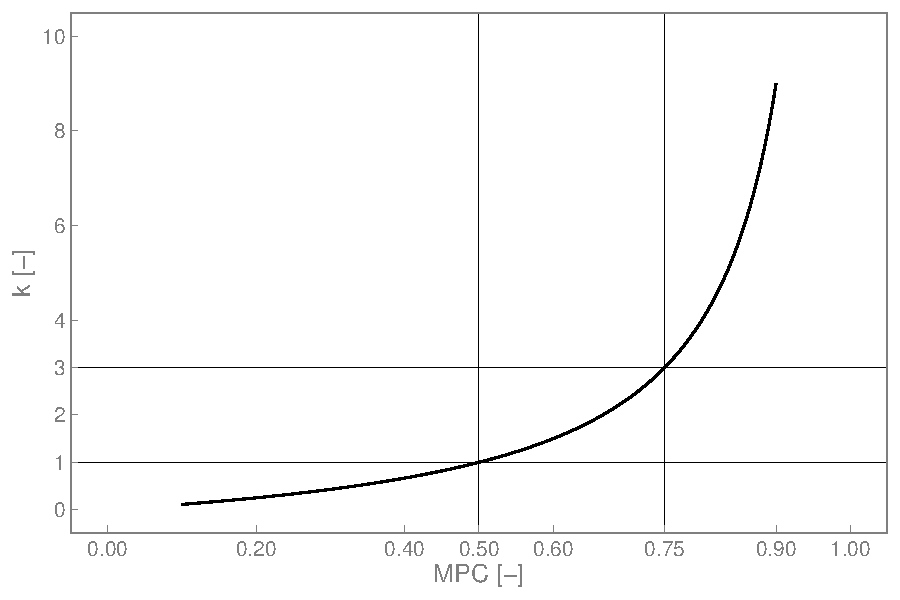
\includegraphics[width=\maxwidth]{figure/k_vs_mpc-1} \caption{The relationship between $\MPC$ and $k$ in Eq.~(\ref{eq:mpc_and_k_converged}).}\label{fig:k_vs_mpc}
\end{figure}

\end{knitrout}



\end{document}
